\documentclass[
12pt, 
english,
onehalfspacing,
headsepline,
]{MastersDoctoralThesis}

\usepackage[utf8]{inputenc}
\usepackage[T1]{fontenc}
\usepackage{palatino}
\usepackage{xcolor}

% Define SFSU brand color
\definecolor{SFSUPurple}{HTML}{442C8B}

% \addbibresource{Chapters/Bibi.bib}

\usepackage[autostyle=true]{csquotes} 
\usepackage{float}
\usepackage{chngcntr}
\counterwithout{figure}{chapter}
\usepackage{subcaption}

\usepackage{graphicx}
% SVG support - requires Inkscape installed and shell-escape enabled
% Compile with: pdflatex -shell-escape main.tex
% Or convert SVGs to PDF manually and use \includegraphics
\usepackage{svg}
% Optimize graphics loading for faster compilation
\graphicspath{{./Docs/Figures/}{./Figures/}{./Figures/Source/}}
% Uncomment the line below to use draft mode (faster compilation, no images)
% \draft
\usepackage{wrapfig}
\usepackage{lscape}
\usepackage{rotating}
\usepackage{epstopdf}

\usepackage[normalem]{ulem}
\useunder{\uline}{\ul}{}

\geometry{
    paper=a4paper,
    inner=3cm,
    outer=3.8cm,
    bindingoffset=.5cm,
    top=2.5cm,
    bottom=2.5cm,
}
\usepackage{indentfirst}

%----------------------------------------------------------------------------------------
%	THESIS INFORMATION
%----------------------------------------------------------------------------------------

% Fix for buggy \thesistitle command in class file
\makeatletter
\RenewDocumentCommand{\thesistitle}{ o m }{
	\IfNoValueTF{#1}{
		\DeclareDocumentCommand{\shorttitle}{}{#2}
	}{
		\DeclareDocumentCommand{\shorttitle}{}{#1}
	}
	\DeclareDocumentCommand{\ttitle}{}{#2}
	\title{#2}  % Also set \title for compatibility
}
\makeatother

\thesistitle[Real-Time Emotion Analysis Platform]{Real-Time Emotion Analysis Platform for Social Media Data}
\supervisor{Dr. Shahrukh Humayoun \& Dr. Jingyi Wang}
\examiner{}
\degree{Master of Science in Computer Science}
\author{Naisarg Halvadiya}
\addresses{}

\subject{Natural Language Processing, Emotion Analysis, Social Media Analytics}
\keywords{Emotion Analysis, NLP, Transformer Models, Real-time Analytics, Social Media, Sentiment Analysis, Data Visualization}

\university{San Francisco State University}
\faculty{College of Science and Engineering}
\department{Department of Computer Science}
\group{Department of Computer Science}

% Configure hyperref - override class defaults after hyperref loads
% Define SFSU Purple in RGB model for hyperref compatibility
\definecolor{SFSUPurpleRGB}{RGB}{68,44,139}
\makeatletter
\AtEndPreamble{%
\hypersetup{
    pdftitle=\@title,
    pdfauthor=\@author,
    pdfkeywords={Emotion Analysis, NLP, Transformer Models, Real-time Analytics, Social Media, Sentiment Analysis, Data Visualization},
    colorlinks=true,
    linkcolor=SFSUPurpleRGB,
    urlcolor=SFSUPurpleRGB,
    citecolor=SFSUPurpleRGB,
    filecolor=SFSUPurpleRGB,
}%
}
\makeatother

\begin{document}

\frontmatter

\let\cleardoublepage\clearpage

\pagestyle{plain}

%----------------------------------------------------------------------------------------
%	TITLE PAGE
%----------------------------------------------------------------------------------------

\begin{singlespacing}

\newgeometry{
    paper=a4paper,
    inner=2cm,
    outer=2.8cm,
    bindingoffset=.5cm,
    top=1.5cm,
    bottom=1.5cm,
    }

\begin{titlepage}
\begin{center}

\vspace*{.06\textheight}

{\scshape\LARGE \textcolor{SFSUPurple}{\univname}\par}\vspace{1.5cm}

\textsc{\Large Master's Thesis}\\[0.5cm]

\HRule \\[0.4cm]

{\huge\bfseries \ttitle\par}\vspace{0.4cm}

\HRule \\[1.5cm]

\begin{flushleft}
\emph{Author:}\\
Naisarg Halvadiya
\end{flushleft}

\begin{flushleft}
\emph{Supervisors:}\\
\href{https://faculty.sfsu.edu/~humayoun/}{\textcolor{SFSUPurple}{Dr. Shahrukh Humayoun}}\\
\href{https://cs.sfsu.edu/people/jingyi-wang}{\textcolor{SFSUPurple}{Dr. Jingyi Wang}}
\end{flushleft}
 
\vfill

\large \textit{A thesis submitted in partial fulfillment of the requirements\\
for the degree of \degreename\\~\\
in the Department of Computer Science}\\[0.3cm]
 
\vfill

{\large \today}\\[4cm]

\end{center}
\end{titlepage}

\restoregeometry

\end{singlespacing}

%----------------------------------------------------------------------------------------
%	DECLARATION
%----------------------------------------------------------------------------------------

\begin{singlespacing}

\begin{declaration}
\addchaptertocentry{\authorshipname}

\noindent I, \authorname, declare that this thesis titled, \enquote{\ttitle} and the work presented in it are my own. I confirm that:

\begin{itemize} 
\item This work was done wholly or mainly while in candidature for a research degree at this University.
\item Where any part of this thesis has previously been submitted for a degree or qualification at this or any other institution, this has been clearly stated.
\item Where I have consulted the published work of others, this is always clearly attributed.
\end{itemize}

\end{declaration}

\end{singlespacing}

%----------------------------------------------------------------------------------------
%	ACKNOWLEDGEMENTS
%----------------------------------------------------------------------------------------

\begin{singlespacing}

\begin{acknowledgements}
\addchaptertocentry{\acknowledgementname}

\setlength{\parskip}{10pt plus 1pt minus 1pt}

I am appreciative of my family's constant encouragement and support during my academic career. Their confidence in my skills has been a continual source of inspiration.

I would like to express my sincere gratitude to my supervisor, Dr. Shahrukh Humayoun, for his invaluable support and flexibility throughout this project. His guidance, patience, and willingness to accommodate various challenges during the research process have been instrumental in the completion of this work.

I would also like to thank the open-source community for making this research feasible. In particular, I am grateful to the developers of D3.js, Hugging Face Transformers, Ollama, Kafka, and various NLP tools and APIs that supported model integration and data processing throughout this work. The collaborative and innovative spirit of the open-source ecosystem has been invaluable to the success of this research.

I would especially like to thank my San Francisco State University peers and colleagues for their insightful comments and discussions, which have enhanced our study.

This thesis reflects not only my own work but also the combined efforts and support of all the individuals listed above. I sincerely appreciate having such an amazing network of support.\\[2cm]

\noindent
Author\\
\authorname

\end{acknowledgements}

\newpage

\end{singlespacing}

%----------------------------------------------------------------------------------------
%	ABSTRACT
%----------------------------------------------------------------------------------------

\begin{singlespacing}

\begin{abstract}
\addchaptertocentry{\abstractname} 

Social media has matured into a shared record of how communities experience the world in real time. Posts arrive with timestamps, locations, and emotions attached, creating a living archive of public mood. The pace of these conversations creates opportunities for real-time analysis that can provide insights as events unfold. This thesis addresses the need for systems that can process, analyze, and visualize emotion data in real-time.

To respond, I reworked the existing pipeline so it behaves more like a listener than a ledger. A tweet agent gathers the ongoing conversation, the processing layer translates each message into a profile of emotions without losing the geographic context, storage keeps the evolving memory, the API shares it immediately, and the interface gives it visual form. Each layer contributes its own perspective, but together they preserve the story of ``who felt what'' across place and time.

The final piece is voice. A generative AI assistant allows someone to ask, in plain language, where emotions are shifting or which region shows the widest divide between optimism and worry. The chatbot answers with narrative context and a chart, closing the gap between complex analytics and human understanding. In the end, the system keeps pace with the public pulse, offering graduate-level rigor while still sounding like a conversation with someone who was actually paying attention.

\end{abstract}

\end{singlespacing}

%----------------------------------------------------------------------------------------
%	TABLE OF CONTENTS / FIGURES
%----------------------------------------------------------------------------------------

\tableofcontents

\listoffigures

%----------------------------------------------------------------------------------------
%	CHAPTERS
%----------------------------------------------------------------------------------------

\mainmatter

\pagestyle{thesis}

% Chapter 1 - Introduction

\chapter{Introduction}

\label{Chapter1}

%----------------------------------------------------------------------------------------

% Define some commands to keep the formatting separated from the content 
\newcommand{\keyword}[1]{\textbf{#1}}
\newcommand{\tabhead}[1]{\textbf{#1}}
\newcommand{\code}[1]{\texttt{#1}}
\newcommand{\file}[1]{\texttt{\bfseries#1}}
\newcommand{\option}[1]{\texttt{\itshape#1}}
\setlength{\parindent}{1.5cm} 

%----------------------------------------------------------------------------------------

Social media platforms have transformed how people communicate, share experiences, and express emotions about events happening around them. Every day, millions of posts are created with timestamps, geographic locations, and rich emotional content, creating an unprecedented dataset for understanding how communities experience and react to events across different regions. This vast stream of data presents both opportunities and challenges for researchers, policy makers, and analysts who seek to understand public sentiment and emotional responses in real-time.

This thesis presents TECVis 2.0, a real-time emotion analysis platform that addresses the need for systems capable of processing, analyzing, and visualizing social media emotion data as it arrives. The platform builds upon the foundation established by TECVis~\cite{tecvis2023}, a visual analytics tool developed in 2019 for comparing emotional reactions to events across geographic locations. While TECVis demonstrated the value of combining emotion analysis with visual analytics, the field has evolved significantly since 2019, presenting opportunities to enhance the system with modern technologies and capabilities.

%----------------------------------------------------------------------------------------

\section{Background and Motivation}

Social media platforms generate enormous volumes of data every second. Twitter alone processes hundreds of millions of tweets daily, each containing text, metadata, and implicit emotional signals. This data represents a real-time record of how people feel about events, policies, products, and experiences. The ability to analyze these emotions in real-time has become increasingly valuable across multiple domains.

Policy makers need to understand public reactions to policy announcements quickly, enabling responsive governance. Crisis coordinators require real-time monitoring of emotional responses during emergencies to allocate resources effectively. Researchers study how different communities respond to the same events, revealing cultural and regional patterns. Marketing teams track brand sentiment across regions to inform campaign strategies. All of these use cases benefit from systems that can process emotion data as it arrives, rather than analyzing historical snapshots days or weeks later.

The field of emotion analysis has advanced significantly since 2019. Transformer-based models have demonstrated substantial improvements in accuracy over lexicon-based methods, while streaming architectures enable real-time processing at scale. Generative AI has opened new possibilities for conversational interfaces that make complex analytics accessible to non-technical users. These advances create opportunities to enhance existing systems while preserving their core value propositions.

%----------------------------------------------------------------------------------------

\section{Problem Statement}

The need for real-time emotion analysis of social media data has grown as platforms generate continuous streams of posts containing rich emotional content. Effective analysis requires systems that can process data as it arrives, accurately detect emotions using modern techniques, provide interactive visualizations for exploration, and enable non-technical users to query data through natural language interfaces. Additionally, systems must scale horizontally to handle the millions of posts generated daily.

A review of existing emotion analysis and visualization platforms, detailed in Chapter 2, reveals that while individual systems have made valuable contributions to specific aspects of emotion analysis and visualization, no existing platform provides a unified solution that combines all the capabilities needed for effective real-time emotion analysis of social media data. Specifically, no existing platform simultaneously provides:

\begin{enumerate}
\item \textbf{Real-time streaming processing.} Existing platforms typically process data in batch mode, which works well for historical analysis but does not support real-time observation of emotional patterns as events unfold. This limitation prevents users from responding to events as they happen, as insights become available only after data collection and processing are complete.

\item \textbf{Modern transformer-based emotion detection.} Existing platforms use lexicon-based methods that were state-of-the-art when developed, achieving approximately 41\% accuracy on benchmark datasets. Modern transformer models can understand context, sarcasm, and nuanced emotional expressions, achieving 84\% accuracy while maintaining reasonable inference speed, but no existing platform has integrated these advances into a complete emotion analysis system.

\item \textbf{Conversational interfaces for data exploration.} Existing platforms require users to interact through predefined visualizations and filters, which works well for users familiar with data visualization but creates barriers for non-technical users. Recent advances in generative AI have created opportunities for conversational interfaces, but no existing emotion analysis platform provides this capability.

\item \textbf{Integrated architecture combining all capabilities.} Individual systems excel in specific areas such as geographic visualization, temporal analysis, or event detection. However, no existing platform combines real-time data processing, modern transformer-based emotion detection, interactive geographic-temporal visualization, and conversational interfaces in a unified architecture.

\item \textbf{Horizontal scalability for high-volume data.} Existing batch processing architectures do not support the horizontal scaling needed to handle the millions of posts generated daily by social media platforms. Streaming architectures that support adding processing components are needed for systems that can grow with data volume.
\end{enumerate}

The absence of a platform that provides this combination of capabilities motivated the development of TECVis 2.0. This system was created to address the need for a unified platform that combines real-time streaming processing, modern transformer-based emotion detection, interactive geographic-temporal visualization, and conversational interfaces, while building upon the valuable foundation established by TECVis and incorporating insights from related work in visual analytics, as discussed in Chapter 2.

%----------------------------------------------------------------------------------------

\section{Research Objectives}

This thesis aims to develop and evaluate a real-time emotion analysis platform that addresses the challenges identified above. The specific research objectives are:

\begin{enumerate}
\item \textbf{Design and implement a streaming architecture} that enables real-time processing of social media data, reducing latency from hours or days to milliseconds while maintaining scalability.

\item \textbf{Evaluate and select optimal emotion detection models} that provide significant accuracy improvements over lexicon-based methods while meeting real-time processing requirements.

\item \textbf{Develop a conversational interface} that enables non-technical users to query emotion data using natural language, making complex analytics accessible without requiring database or visualization expertise.

\item \textbf{Integrate modern visualization techniques} that extend existing capabilities while preserving the geographic and temporal comparison features that made TECVis valuable.

\item \textbf{Evaluate system performance} across multiple dimensions including latency, throughput, accuracy, and user experience, demonstrating that the platform achieves its design goals.
\end{enumerate}

These objectives guide the design, implementation, and evaluation of TECVis 2.0, ensuring that the system addresses real needs while advancing the state of the art in emotion analysis and visual analytics.

%----------------------------------------------------------------------------------------

\section{Contributions}

This thesis makes several contributions to the fields of emotion analysis, visual analytics, and real-time data processing:

\begin{enumerate}
\item \textbf{Real-time streaming architecture.} TECVis 2.0 implements a Kafka-based streaming pipeline that processes social media data as it arrives, enabling insights within seconds rather than hours or days. This architecture supports horizontal scaling, allowing the system to handle increasing data volumes.

\item \textbf{Improved emotion detection accuracy.} The system replaces lexicon-based methods with transformer models, achieving 84\% accuracy compared to 41\% with previous methods. An evaluation framework demonstrates that DistilRoBERTa-Emotion provides the optimal balance between accuracy and speed for real-time applications.

\item \textbf{Conversational data exploration.} A generative AI chatbot enables users to query emotion data using natural language, translating questions to SQL, executing queries, selecting appropriate visualizations, and generating natural language summaries. This makes complex analytics accessible to non-technical users.

\item \textbf{Enhanced visualization capabilities.} The platform extends TECVis's visualization features with horizon charts for temporal analysis, difference charts for state comparisons, and dynamic chart selection based on query intent.

\item \textbf{Privacy-preserving design.} The chatbot runs on local LLMs (Ollama), keeping all queries and results on the user's machine. This design choice prioritizes privacy while maintaining the benefits of conversational interfaces.

\item \textbf{Comprehensive evaluation framework.} The thesis provides quantitative evaluation of system performance, model accuracy, chatbot effectiveness, and user experience, demonstrating that the platform achieves its design goals.
\end{enumerate}

These contributions demonstrate that it is possible to modernize existing systems without discarding their core value, while adding new capabilities that address evolving user needs and industry capabilities.

%----------------------------------------------------------------------------------------

\section{Thesis Structure}

This thesis is organized into seven chapters that present the research in a logical progression:

\begin{itemize}
\item \textbf{Chapter 2: Related Work} reviews existing research in visual analytics, emotion analysis systems, geographic-temporal visualization, real-time processing, and conversational interfaces. This chapter establishes the foundation for understanding how TECVis 2.0 relates to and builds upon previous work.

\item \textbf{Chapter 3: Previous System and Dataset} describes the TECVis system that served as the foundation for this work, including its architecture, data collection methods, and the dataset it processed. This chapter provides context for understanding how TECVis 2.0 enhances the original system.

\item \textbf{Chapter 4: System Architecture} presents TECVis 2.0's architecture, beginning with motivation and contributions, then describing the model selection process, data flow, components, and design decisions that enable real-time processing and scalability.

\item \textbf{Chapter 5: System Description} details the implementation of each component and demonstrates how users interact with the system through screenshots and walkthroughs. This chapter shows the system in action, from data ingestion to visualization rendering.

\item \textbf{Chapter 6: Evaluation} presents performance metrics, user experience evaluation, and comparisons with the previous TECVis system. This chapter demonstrates that TECVis 2.0 achieves its design goals across multiple dimensions.

\item \textbf{Chapter 7: Conclusion and Future Work} summarizes the contributions, reflects on insights gained, and outlines directions for future research and development.
\end{itemize}

Throughout this thesis, the focus is on making emotion analysis accessible, real-time, and interactive, while building upon the valuable foundation established by TECVis and incorporating modern technologies that address evolving user needs.

%----------------------------------------------------------------------------------------

\let\cleardoublepage\clearpage

% Chapter 2 - Related Work

\chapter{Related Work}
\label{Chapter2}

%----------------------------------------------------------------------------------------

This chapter reviews related work in visual analytics for social media, emotion analysis systems, and interactive visualization platforms. The review focuses on published research systems and platforms that address similar challenges to those addressed by TECVis 2.0.

%----------------------------------------------------------------------------------------

\section{Visual Analytics Foundations}

Visual analytics combines automated analysis techniques with interactive visualizations to enable human understanding of complex data \cite{thomas2005visual}. The field emerged from the recognition that purely automated analysis often misses important patterns that humans can identify through visual exploration.

Keim et al. \cite{keim2013visual} surveyed visual analytics approaches for social media, highlighting the importance of temporal, geographic, and network visualizations. They emphasized that effective social media analytics requires combining multiple visualization techniques to capture different aspects of the data.

%----------------------------------------------------------------------------------------

\section{Social Media Sentiment and Emotion Visualization Systems}

Several research systems have been developed for visualizing sentiment and emotions in social media data. This section reviews published platforms that address similar challenges.

\subsection{OpinionSeer}

OpinionSeer \cite{wu2009opinionseer} is an interactive visualization system for analyzing customer opinions. The system's unique strength lies in its radial visualization approach, which effectively displays opinion distributions across multiple dimensions simultaneously. The system provides intuitive filtering capabilities that enable users to explore opinion data interactively.

\begin{figure}[htbp]
\centering
\includesvg[width=0.8\textwidth]{Figures/Source/OpinionSeer}
\caption{OpinionSeer architecture (Taken from Wu et al.~\cite{wu2009opinionseer})}
\label{fig:opinionseer}
\end{figure}

While OpinionSeer demonstrates effective techniques for visualizing opinion distributions, it focuses on product reviews rather than social media streams. The system processes data in batch mode, which means it cannot provide real-time insights as new opinions arrive. Additionally, OpinionSeer does not incorporate geographic or temporal dimensions, limiting its ability to analyze how opinions vary across locations and time periods. These limitations motivated the need for a system that combines real-time processing with geographic-temporal visualization for social media emotion analysis.

\subsection{TwitInfo}

TwitInfo \cite{marcus2011twitinfo} is a system for visualizing Twitter event streams in real-time. The system's unique strength is its event detection and peak identification capabilities, which automatically identify significant events by detecting spikes in tweet volume. TwitInfo visualizes temporal patterns effectively, enabling users to understand how events unfold over time through interactive timeline visualizations.

\begin{figure}[htbp]
\centering
\includesvg[width=0.8\textwidth]{Figures/Source/TwitInfo}
\caption{TwitInfo architecture (Taken from Marcus et al.~\cite{marcus2011twitinfo})}
\label{fig:twitinfo}
\end{figure}

TwitInfo demonstrates effective techniques for processing and visualizing real-time social media streams, but it focuses on event detection and volume analysis rather than emotion analysis. The system does not provide emotion classification or geographic visualization capabilities. While TwitInfo processes data in real-time, it does not incorporate modern transformer-based emotion detection models, limiting its ability to understand the emotional content of tweets. These gaps motivated the development of a system that combines real-time event processing with comprehensive emotion analysis and geographic visualization.

\subsection{EmoViz}

EmoViz \cite{emoviz2014} provides geographic visualization of emotions extracted from social media posts. The system's unique contribution is its ability to map emotions to geographic locations, enabling users to understand regional emotional patterns through interactive maps. EmoViz demonstrates how geographic visualization can reveal spatial patterns in emotional responses.

\begin{figure}[htbp]
\centering
\includesvg[width=0.8\textwidth]{Figures/Source/EmoViz}
\caption{EmoViz architecture (Taken from Wang et al.~\cite{emoviz2014})}
\label{fig:emoviz}
\end{figure}

While EmoViz excels at geographic emotion visualization, it relies on lexicon-based emotion detection methods that achieve limited accuracy. The system processes data in batch mode rather than providing real-time streaming capabilities. Additionally, it does not incorporate conversational interfaces, requiring users to interact through predefined visualizations and filters. These limitations highlight the need for a system that combines real-time processing, modern transformer-based emotion detection, and conversational interfaces with geographic-temporal visualization.

%----------------------------------------------------------------------------------------

\section{Emotion Analysis in Social Media}

Emotion analysis in social media has been addressed through various approaches, from lexicon-based methods to modern transformer models.

\subsection{Lexicon-Based Approaches}

Early emotion analysis systems relied on lexicons that map words to emotions. The NRC Emotion Lexicon \cite{mohammad2013nrc} maps approximately 14,000 words to eight emotions based on Plutchik's wheel of emotions \cite{plutchik1980emotion}. VADER \cite{hutto2014vader} was specifically designed for social media text, handling slang, emoticons, and punctuation-based emphasis.

These lexicon-based approaches have advantages: they are fast, interpretable, and require no training data. They analyze words as independent tokens, which works well for straightforward emotional expressions. Transformer models build upon this foundation by understanding context, sarcasm, and nuanced emotional expressions.

\subsection{Neural Network Approaches}

Recurrent Neural Networks (RNNs) and Long Short-Term Memory (LSTM) networks improved emotion detection by capturing sequential dependencies in text \cite{hochreiter1997long}. These models process text sequentially, which provides strong performance for many tasks. Transformer models process entire sequences in parallel, enabling faster processing and better handling of long-range context.

\subsection{Transformer-Based Approaches}

The transformer architecture \cite{vaswani2017attention} revolutionized natural language processing by processing entire sequences in parallel through self-attention mechanisms. BERT \cite{devlin2018bert} and RoBERTa \cite{liu2019roberta} applied transformers to language understanding, achieving state-of-the-art performance on various NLP tasks.

For emotion analysis, transformer models have shown significant improvements over lexicon-based methods. DistilRoBERTa-Emotion \cite{hartmann2023emotion} provides transformer-level accuracy while maintaining reasonable inference speed through model distillation \cite{sanh2019distilbert}.

\subsection{Evaluation of Emotion Models}

Several studies have evaluated emotion detection models on social media datasets. GoEmotions \cite{go2018emotions} introduced a dataset of fine-grained emotions from Reddit and evaluated various models. The Kaggle Twitter Emotion Dataset provides a large-scale benchmark for emotion classification on Twitter data.

These evaluations consistently show that transformer-based models outperform lexicon-based methods, though the choice between accuracy and speed depends on the application requirements.

%----------------------------------------------------------------------------------------

\section{Geographic and Temporal Visualization}

Several research systems have focused on visualizing social media data across geographic and temporal dimensions.

\subsection{Geographic Visualization Systems}

GeoSocial \cite{pat2015geosocial} provides geosocial search capabilities that enable users to find locations based on geotagged social media posts. The system's unique strength is its two-step process: first, quickly finding relevant areas using an indexed partition of space, and second, applying clustering on discovered areas to present more accurate results. The system demonstrates how geotagged posts can be used for geographic search, showing where people talk about different topics. For example, searches for terms like "jogging" or "sunset" can indicate popular locations associated with those activities.

\begin{figure}[htbp]
\centering
\includesvg[width=0.8\textwidth]{Figures/Source/GeoSocial}
\caption{GeoSocial architecture (Taken from Pat et al.~\cite{pat2015geosocial})}
\label{fig:geosocial}
\end{figure}

While GeoSocial excels at geographic search based on social media content, it focuses on location discovery rather than emotion analysis. The system processes data in batch mode and does not incorporate real-time streaming capabilities or modern transformer-based emotion detection models. Additionally, it lacks temporal visualization components and conversational interfaces. These limitations highlight the need for a system that combines geographic visualization with real-time emotion analysis, temporal exploration, and conversational interfaces.

\subsection{Temporal Visualization Techniques}

Temporal visualization helps users understand how emotions evolve over time. Horizon charts \cite{healy2010horizon} provide an effective way to visualize multiple time series in a compact format. These charts stack colored bands to show intensity, making it easy to spot peaks and trends across multiple dimensions simultaneously. The technique's unique strength is its ability to display many time series in a space-efficient manner while maintaining readability.

Sparklines \cite{tufte2006sparklines} provide another approach to temporal visualization, showing trends in a compact format. These visualizations are useful for displaying multiple time series simultaneously in minimal space, enabling users to quickly identify patterns across many dimensions.

While these temporal visualization techniques are effective, they are typically applied to batch-processed data rather than real-time streams. They do not incorporate geographic dimensions or emotion analysis capabilities. Additionally, these techniques require users to interact through predefined interfaces rather than conversational queries. These limitations motivated the need for a system that combines effective temporal visualization with real-time processing, geographic analysis, and conversational interfaces.

%----------------------------------------------------------------------------------------

\section{Real-Time Data Processing}

Real-time emotion analysis requires streaming data processing architectures. Apache Kafka \cite{kreps2011kafka} has become a standard for building real-time data pipelines, enabling decoupled producers and consumers that can scale independently. Kafka's unique strength is its ability to handle high-throughput, low-latency data streams while maintaining durability and fault tolerance. However, existing systems that utilize Kafka for social media analysis typically focus on general data processing rather than emotion analysis, and they do not incorporate modern transformer-based emotion detection models or conversational interfaces.

%----------------------------------------------------------------------------------------

\section{Conversational Interfaces for Data Exploration}

Recent advances in generative AI have enabled conversational interfaces for data exploration. Natural Language to SQL (NL2SQL) translation allows users to query databases using plain English \cite{zhong2017seq2sql}, making database queries accessible to non-technical users. Chart suggestion systems analyze query results and recommend appropriate visualizations \cite{mackinlay2007show}, automatically selecting the most effective visualization type based on data characteristics and query intent.

However, existing conversational interfaces for data exploration typically focus on static datasets rather than real-time streaming data. They do not incorporate emotion analysis or geographic-temporal visualization capabilities. Additionally, many systems require cloud-based LLM services, which may raise privacy concerns for sensitive data. These gaps motivated the need for a system that combines conversational interfaces with real-time emotion analysis, geographic-temporal visualization, and privacy-preserving local LLM execution.

%----------------------------------------------------------------------------------------

\section{Summary}

This chapter has reviewed related work in visual analytics for social media, emotion analysis systems, geographic-temporal visualization, real-time processing, and conversational interfaces. The review examined published research systems and platforms, highlighting each system's unique contributions while identifying gaps that motivated the development of TECVis 2.0.

The review reveals that while individual systems excel in specific areas, such as OpinionSeer's radial visualizations, TwitInfo's event detection, EmoViz's geographic emotion visualization, and GeoSocial's location-based search, no existing platform provides a unified solution that combines all these capabilities.

Specifically, existing platforms lack one or more of the following: real-time streaming processing, modern transformer-based emotion detection, geographic-temporal visualization, and conversational interfaces. The absence of a platform that integrates all these capabilities motivated the development of TECVis 2.0, which combines real-time streaming architecture, modern transformer-based emotion detection, comprehensive geographic-temporal visualization, and privacy-preserving conversational interfaces in a unified system.

The next chapter describes the TECVis system in detail, providing context for understanding how TECVis 2.0 builds upon and extends this foundation.

%----------------------------------------------------------------------------------------
 
% Chapter 3 - Previous System and Dataset

\chapter{Previous System and Dataset}
\label{Chapter3}

%----------------------------------------------------------------------------------------

This chapter describes the TECVis system that served as the foundation for this work, including its architecture, data collection methods, and the dataset it processed.

%----------------------------------------------------------------------------------------

\section{The TECVis System}

TECVis \cite{tecvis2023} was developed between 2019 and 2021 as a visual analytics tool for comparing emotional reactions to events across geographic locations within the United States. The system focused on analyzing COVID-19 related tweets from US states to understand how different regions reacted to pandemic-related announcements and events.

\subsection{Architecture}

Figure~\ref{fig:tecvis_old} shows the original TECVis architecture.

\begin{figure}[htbp]
\centering
\includesvg[width=0.95\textwidth]{Figures/Source/tecvis_1.0}
\caption{TECVis Original Architecture (2019): Batch processing pipeline from Twitter scraping to visualization.}
\label{fig:tecvis_old}
\end{figure}

The TECVis pipeline operated in batch mode:

\begin{enumerate}
\item \textbf{Data collection.} Researchers scraped tweets using the Twitter API, focusing on COVID-19 related keywords such as ``COVID-19,'' ``coronavirus,'' ``pandemic,'' and ``lockdown.'' The collection process gathered tweets with geographic location information, enabling state-level analysis.

\item \textbf{Storage.} Tweets were stored as CSV files containing the original text, timestamp, location information (state codes), and metadata. The system processed these files in batches rather than real-time streams.

\item \textbf{Preprocessing.} Scripts cleaned the text, removing URLs, normalizing characters, handling special cases, and filtering out retweets or duplicate content. This preprocessing step prepared the text for emotion analysis.

\item \textbf{Emotion analysis.} Each tweet was processed through two emotion classifiers:
\begin{itemize}
\item \textbf{NRC Emotion Lexicon} \cite{mohammad2013nrc}: Maps words to eight emotions (anger, fear, anticipation, trust, surprise, sadness, joy, disgust) based on Plutchik's wheel of emotions. The lexicon-based approach counts emotion-associated words in each tweet and assigns scores accordingly.
\item \textbf{VADER} \cite{hutto2014vader}: Provides sentiment scores ranging from -1 (negative) to +1 (positive), specifically designed for social media text. VADER handles slang, emoticons, and punctuation-based emphasis that are common in Twitter posts.
\end{itemize}

These lexicon-based methods were state-of-the-art for social media emotion analysis in 2019, offering fast processing and interpretable results without requiring training data or computational resources.

\item \textbf{Data storage.} Results were stored as another CSV file with emotion scores and sentiment classifications. The aggregated data included state-level averages for each emotion category, enabling geographic comparison.

\item \textbf{Visualization.} A React frontend with D3.js visualizations fetched data from a Node.js API and displayed it in interactive dashboards. The visualization layer provided the dot plot and tornado chart views that enabled users to explore emotional patterns across states.
\end{enumerate}

\subsection{Visualization Features}

TECVis provided two main visualization types:

\begin{itemize}
\item \textbf{Dot Plot.} Showed emotion scores across all US states. Each dot represented a state's average score for a specific emotion, enabling geographic comparison. Users could filter by emotion type and observe which states showed higher or lower scores for specific emotions.

\item \textbf{Tornado Chart.} Compared two states side-by-side, with bars extending left and right from a center axis to show which state scored higher on each emotion. This visualization made it easy to identify differences in emotional responses between states.
\end{itemize}

\subsection{Strengths of TECVis}

TECVis demonstrated several valuable contributions:

\begin{itemize}
\item \textbf{Geographic comparison.} The system effectively visualized how different states reacted to the same events, revealing regional patterns in emotional responses to COVID-19 related news and announcements.

\item \textbf{Temporal tracking.} Users could observe how emotions evolved over time, though the batch processing meant updates were periodic rather than real-time. The system processed data in weekly or monthly batches.

\item \textbf{Simplicity.} The architecture was straightforward, making it easy to understand and reproduce. The lexicon-based emotion detection required no model training or fine-tuning.

\item \textbf{Low computational cost.} Lexicon-based methods required minimal computational resources, allowing the system to process large datasets on standard hardware without GPU acceleration.
\end{itemize}

The system successfully processed 574,806 tweets related to COVID-19, providing researchers with insights into how different regions responded to pandemic-related events.

%----------------------------------------------------------------------------------------

\section{The TECVis Dataset}

The TECVis system processed a dataset of 574,806 tweets collected during the COVID-19 pandemic, focusing exclusively on data from the United States. This dataset served as the foundation for understanding how different US states reacted to pandemic-related events.

\subsection{Data Collection}

Tweets were collected using the Twitter API, focusing on COVID-19 related keywords:
\begin{itemize}
\item Primary keywords: ``COVID-19,'' ``coronavirus,'' ``pandemic,'' ``lockdown''
\item Collection period: 2019-2021 (during the height of the COVID-19 pandemic)
\item Geographic focus: United States, with state-level location information
\item Language: English-language tweets
\end{itemize}

\subsection{Data Characteristics}

The TECVis dataset had several characteristics that influenced the system design:

\begin{itemize}
\item \textbf{Event-driven content.} Tweets focused on COVID-19 related events, announcements, and news, creating a coherent thematic dataset for analysis.

\item \textbf{Geographic distribution.} Tweets included state-level location information, enabling the geographic comparison features that were central to TECVis's value proposition.

\item \textbf{Temporal span.} The dataset covered multiple months during the pandemic, allowing researchers to observe how emotional responses evolved as the situation changed.

\item \textbf{Informal language.} Like all social media data, the tweets contained slang, abbreviations, and informal grammar, which the lexicon-based methods (NRC and VADER) were designed to handle.

\item \textbf{High volume.} With over 574,000 tweets, the dataset was large enough to provide statistically meaningful state-level aggregations while remaining manageable for batch processing.
\end{itemize}

\subsection{Characteristics of Lexicon-Based Methods}

TECVis successfully processed this dataset using lexicon-based emotion detection methods (NRC and VADER). These methods have specific characteristics that influenced the system design:

\begin{itemize}
\item \textbf{Word-level analysis.} Lexicon methods treat words as independent tokens, which works well for straightforward emotional expressions but may miss contextual nuances that require understanding sentence structure and meaning.

\item \textbf{Static vocabulary.} The emotion lexicons use fixed word lists, which work well for established terminology and may require updates for new slang or emerging language patterns.

\item \textbf{Direct word mapping.} Words are mapped directly to emotions, providing interpretable results that are easy to understand and verify.

\item \textbf{Rule-based processing.} Lexicon methods use predefined rules rather than learning from data, which provides consistent results and requires no training data.
\end{itemize}

As transformer-based models became available, opportunities emerged to enhance emotion detection with models that can understand context and learn from data. TECVis 2.0 incorporates these advances while preserving the interpretability and efficiency that made lexicon-based methods valuable for the original system.

%----------------------------------------------------------------------------------------

\section{Summary}

This chapter has described the TECVis system that provided the foundation for this work. TECVis demonstrated the value of combining emotion analysis with visual analytics for geographic and temporal comparison, successfully processing over 574,000 COVID-19 related tweets using lexicon-based methods (NRC Emotion Lexicon and VADER) that were state-of-the-art in 2019. The system's batch processing architecture and visualization features provided valuable insights into regional emotional responses to pandemic events.

As the field advanced, opportunities emerged to enhance lexicon-based methods with transformer models that can understand context and learn from data. The next chapter describes the architecture of TECVis 2.0, which incorporates modern transformer-based emotion detection and real-time processing capabilities.

%----------------------------------------------------------------------------------------

% Chapter 4 - System Architecture

\chapter{System Architecture}
\label{Chapter4}

%----------------------------------------------------------------------------------------

This chapter presents TECVis 2.0, a real-time emotion analysis platform that builds upon the original TECVis system while incorporating modern technologies and preserving its core strengths. Like TECVis, TECVis 2.0 focuses exclusively on analyzing social media data from the United States, enabling state-level geographic comparison of emotional responses. The chapter begins by establishing the motivation for this work, then describes the architecture and design decisions that enable real-time processing, improved accuracy, and conversational interfaces.

%----------------------------------------------------------------------------------------

\section{Motivation and Contributions}

The original TECVis system demonstrated the value of combining emotion analysis with visual analytics for geographic and temporal comparison. As described in Chapter 3, the system used lexicon-based emotion detection methods (NRC and VADER) that were state-of-the-art in 2019. As the field advanced, transformer-based models became available that could understand context, adapt to new language patterns, and learn from data, creating opportunities to enhance emotion detection capabilities while preserving the system's core strengths.

TECVis 2.0 incorporates three key enhancements:

\begin{enumerate}
\item \textbf{Real-time processing.} Replaces batch processing with a streaming architecture using Apache Kafka, enabling continuous data flow and reducing latency from hours or days to milliseconds.

\item \textbf{Enhanced emotion detection.} Incorporates transformer models alongside the lexicon-based foundation, achieving 84\% accuracy compared to 41\% with VADER while maintaining reasonable inference speed for real-time applications.

\item \textbf{Conversational interface.} Introduces a generative AI chatbot that enables users to query data using natural language, making complex analytics accessible to non-technical users without requiring database or visualization expertise.
\end{enumerate}

These contributions build upon TECVis's foundation while incorporating modern technologies that address evolving user needs and industry capabilities.
 
%----------------------------------------------------------------------------------------

\section{Model Selection and Evaluation}

Before designing the architecture, an evaluation framework was developed to select the optimal emotion detection model for real-time processing. The goal was to find a model that significantly improved accuracy over lexicon-based methods while maintaining inference speed suitable for streaming applications.

\subsection{Evaluation Framework}

The Kaggle Twitter Emotion Dataset, containing 416,809 tweets labeled with six emotions (sadness, joy, love, anger, fear, and surprise), served as the benchmark for model comparison. This dataset provides a large-scale, real-world benchmark for emotion classification on Twitter data, making it ideal for evaluating models intended for social media analysis.

The evaluation framework measured three key metrics:
\begin{itemize}
\item \textbf{Accuracy.} The percentage of correctly classified emotions, indicating how well the model performs on the task.
\item \textbf{F1 Score.} A balanced metric considering both precision and recall, especially important for multi-class emotion classification where classes may be imbalanced.
\item \textbf{Inference Speed.} The time required to process each tweet, critical for real-time applications where latency matters.
\end{itemize}

\subsection{Model Comparison}

Multiple models were evaluated on this dataset:

\begin{itemize}
\item \textbf{VADER} (baseline): The lexicon-based method used in TECVis, achieving 41.2\% accuracy. This served as the baseline representing the previous system's capabilities.

\item \textbf{GoEmotions-Electra}: Google's emotion classifier based on the Electra architecture, achieving 47.5\% accuracy with inference time of 0.063 seconds per tweet.

\item \textbf{DistilRoBERTa-Emotion}: A distilled transformer model \cite{hartmann2023emotion}, achieving 84.0\% accuracy with inference time of 0.048 seconds per tweet.

\item \textbf{RoBERTa-Large}: Full RoBERTa architecture \cite{liu2019roberta}, achieving 84.0\% accuracy with inference time of 0.049 seconds per tweet.
\end{itemize}

\subsection{Selection Rationale}

DistilRoBERTa-Emotion was selected for TECVis 2.0 because it provided the optimal balance between accuracy and speed. The model achieved 84\% accuracy, more than double the 41\% achieved by VADER, while maintaining inference speed (0.048s per tweet) suitable for real-time processing. This represents a significant improvement in emotion detection quality while meeting the performance requirements of a streaming architecture.

The evaluation demonstrated that transformer-based models can achieve substantial accuracy improvements over lexicon-based methods, validating the decision to modernize the emotion detection pipeline. This model selection informed the architecture design, ensuring the NLP pipeline could handle real-time processing requirements.

%----------------------------------------------------------------------------------------

\newpage
\section{Architecture Overview}

Figure~\ref{fig:new_architecture} shows the TECVis 2.0 architecture.

\begin{figure}[htbp]
\centering
\includesvg[width=0.95\textwidth]{Figures/Source/tecvis_2.0}
\caption{TECVis 2.0 Architecture: Real-time streaming pipeline with Kafka, NLP processing, and conversational interface.}
\label{fig:new_architecture}
\end{figure}

The architecture follows a streaming pattern where data flows continuously from ingestion through processing to visualization. Each component operates independently, enabling horizontal scaling and fault tolerance. This design contrasts with TECVis's batch processing approach, where data was collected, processed, and then visualized in discrete stages.

%----------------------------------------------------------------------------------------

\section{Data Ingestion Layer}

The data ingestion layer is responsible for collecting and introducing social media data into the system. This layer handles the initial entry point for all data, ensuring that tweets from US states are captured and prepared for downstream processing. The layer consists of a tweet generation agent and a message broker that coordinates data flow.

\subsection{Tweet Generation Agent}

For this proof-of-concept, a tweet generation agent simulates real-time social media activity. The agent uses Ollama to generate realistic tweet text based on configurable keywords, assigns US state locations, timestamps each message, and publishes tweets to Kafka at configurable intervals.

This component is intentionally modular. The architecture allows swapping the agent with X's streaming API when production access becomes available, without requiring changes to other components. This design decision ensures the system can transition from proof-of-concept to production without architectural changes.

\subsection{Apache Kafka Message Broker}

Apache Kafka \cite{kreps2011kafka} serves as the message broker, decoupling producers from consumers. This design provides several benefits:

\begin{itemize}
\item \textbf{Asynchronous processing.} Producers and consumers operate independently, preventing bottlenecks and enabling different processing speeds.

\item \textbf{Scalability.} Multiple consumers can process messages in parallel, increasing throughput as data volume grows.

\item \textbf{Fault tolerance.} If a consumer encounters issues, messages remain in Kafka and can be reprocessed when the consumer recovers.

\item \textbf{Buffering.} Kafka buffers messages, handling temporary spikes in production or consumption rates without data loss.
\end{itemize}

The agent publishes tweets to a Kafka topic. Two consumers subscribe to this topic, each handling a different aspect of processing, enabling parallel processing and independent scaling.

%----------------------------------------------------------------------------------------

\section{Data Processing Layer}

The data processing layer transforms raw social media data into enriched records with emotion and sentiment classifications. This layer operates on streaming data from the ingestion layer, processing tweets in real-time as they arrive. The layer consists of two parallel consumers that handle different aspects of data processing, enabling independent scaling and fault tolerance.

\subsection{Raw Data Consumer}

The first consumer stores raw tweet data immediately upon receipt. This separation ensures that raw data is preserved, even if the NLP pipeline experiences delays or requires reprocessing. It also enables reprocessing of historical data if analysis methods change, providing flexibility for future improvements.

\subsection{NLP Consumer}

The second consumer processes tweets through the emotion detection pipeline. It preprocesses text, runs emotion detection using DistilRoBERTa-Emotion, runs sentiment classification using Twitter-RoBERTa \cite{cardiffnlp2023sentiment}, and stores enriched records with emotion scores and sentiment labels.

The NLP consumer processes tweets independently of the raw data consumer, allowing the system to handle different processing speeds and enabling independent scaling of each component. This design enables the system to maintain real-time processing even if one component experiences delays.

%----------------------------------------------------------------------------------------

\section{NLP Pipeline}

The NLP pipeline performs natural language processing on tweet text to extract emotions and sentiment. This pipeline transforms raw text into structured emotion scores and sentiment classifications that enable downstream analysis and visualization. The pipeline consists of preprocessing, emotion detection, and sentiment classification stages, each optimized for real-time processing of US social media data.

\subsection{Preprocessing}

Before model inference, the pipeline cleans tweet text: removing URLs, extracting words from hashtags, expanding contractions, and normalizing repeated characters. This preprocessing improves model performance by presenting clean, normalized text to the transformer models.

\subsection{Emotion Detection}

DistilRoBERTa-Emotion analyzes each tweet and returns probability scores for seven emotions: anger, disgust, fear, joy, sadness, surprise, and neutral. The model processes the entire tweet in parallel through self-attention mechanisms, returning probability distributions over emotion categories. All emotion scores are stored, not just the dominant emotion, enabling nuanced analysis and supporting visualization of emotion distributions.

\subsection{Sentiment Classification}

Cardiff NLP's Twitter-RoBERTa classifies each tweet as positive, negative, or neutral. This three-way classification complements the seven-way emotion classification, providing both fine-grained emotion analysis and broad sentiment categorization. The combination enables users to explore data at different levels of granularity.

\subsection{Performance}

The NLP pipeline processes tweets in approximately 0.05 seconds each on GPU, or 0.15 seconds on CPU. This performance meets the real-time processing requirements while providing the accuracy improvements demonstrated in the model evaluation.

%----------------------------------------------------------------------------------------

\section{Data Storage Layer}

The data storage layer provides persistent storage for both raw tweets and processed emotion data. This layer enables efficient querying of historical data, supports real-time dashboard updates, and maintains state-level aggregations for fast geographic analysis. The layer uses PostgreSQL as the primary database, with optimized indexing strategies for common query patterns across US state data.

\subsection{PostgreSQL Database}

PostgreSQL stores both raw tweets and processed emotion data. The database schema includes raw tweet data, emotion scores, sentiment classifications, and pre-computed state-level and time-based aggregations for fast dashboard queries.

\subsection{Indexing Strategy}

PostgreSQL indexes are optimized for common query patterns: timestamp indexes for time-range queries, state code indexes for geographic filtering, dominant emotion indexes for emotion filtering, and composite indexes for multi-filter queries. These indexes ensure that dashboard queries execute in 10-50 milliseconds, even with millions of rows, and chatbot SQL queries execute in under 100 milliseconds.

%----------------------------------------------------------------------------------------

\section{API Layer}

The API layer provides programmatic access to processed emotion data for the frontend and chatbot components. This layer serves aggregated data by state, time range, and emotion type, enabling efficient data retrieval for visualizations and queries. The layer consists of a REST API for standard HTTP requests and Server-Sent Events for real-time streaming updates.

\subsection{REST API}

A REST API provides endpoints for dashboard data, time series data, comparison data, and metadata. The API serves aggregated emotion scores by state, time range, and emotion type, enabling the frontend to fetch data efficiently.

\subsection{Server-Sent Events (SSE)}

For real-time updates, the API uses Server-Sent Events to stream new data to the frontend as it arrives. This enables the dashboard to update automatically without requiring user refresh or polling, providing a real-time experience that matches the streaming architecture.

%----------------------------------------------------------------------------------------

\section{Visualization Layer}

The visualization layer presents emotion data through interactive charts and maps that enable users to explore patterns across US states. This layer combines inherited visualizations from TECVis with new visualization types that extend the platform's capabilities. The layer is built with React and uses D3.js and Recharts for rendering interactive visualizations.

\subsection{Frontend Architecture}

The frontend is built with React and uses D3.js and Recharts for visualizations. The architecture separates data fetching, state management, and visualization rendering, enabling modular development and maintenance.

\subsection{Inherited Visualizations}

The platform inherits TECVis's core visualizations: the dot plot for geographic comparison and the tornado chart for state-to-state comparison. These visualizations are preserved to maintain continuity with the original system while benefiting from the improved data quality provided by transformer-based emotion detection.

\subsection{Enhanced Visualizations}

New visualizations extend the platform's capabilities: horizon charts for temporal emotion intensity, difference charts for state comparisons, and dynamic chart selection by the chatbot based on query results and user intent.

%----------------------------------------------------------------------------------------

\section{Chatbot Architecture}

The chatbot architecture enables users to query emotion data using natural language, making complex analytics accessible without requiring database or visualization expertise. This architecture translates natural language questions into SQL queries, executes them against the database, selects appropriate visualizations, and generates natural language summaries. The architecture runs entirely on local LLMs to preserve privacy, keeping all queries and results on the user's machine.

\subsection{Local LLM Runtime}

The chatbot runs on Ollama, a local large language model runtime. This design choice prioritizes privacy: all queries and results remain on the user's machine, making the system suitable for sensitive or proprietary analysis. Ollama supports multiple models, with Mistral used for SQL generation and chart selection.

\subsection{NL2SQL Translation}

When a user asks a natural language question, the system analyzes the question to understand intent, maps location names to state codes, maps temporal references to date ranges, generates valid PostgreSQL syntax using the database schema, and validates the SQL query for common errors. The prompt includes the database schema, example queries, and explicit rules for PostgreSQL syntax.

\subsection{Chart Suggestion Agent}

After query execution, a chart suggestion agent analyzes the results and selects an appropriate visualization based on data structure, user intent, and column patterns. The agent selects from available chart types: line charts for time series, stacked bar charts for composition, grouped bar charts for comparison, radar charts for multi-dimensional profiles.

\subsection{Response Generation}

After rendering the visualization, the chatbot generates a natural language summary explaining what the data shows. This narrative layer helps users understand the results without needing to interpret charts themselves, making complex analytics accessible to non-technical users.

%----------------------------------------------------------------------------------------

\section{Design Principles}

The architecture follows several design principles:

\begin{itemize}
\item \textbf{Modularity.} Components are decoupled, enabling independent development, testing, and deployment.

\item \textbf{Scalability.} The streaming architecture enables horizontal scaling by adding consumers or API instances.

\item \textbf{Fault tolerance.} Kafka buffers messages, and consumers can recover from interruptions without data loss.

\item \textbf{Privacy.} Local LLM runtime keeps queries and results private.

\item \textbf{Extensibility.} The architecture supports adding new visualizations, data sources, or analysis methods without major restructuring.
\end{itemize}

%----------------------------------------------------------------------------------------

\section{Summary}

This chapter presented TECVis 2.0's architecture, including motivation, contributions, and model selection. Transformer-based models achieved substantial accuracy improvements over lexicon-based methods. The streaming architecture enables real-time processing, while modular design supports scalability and extensibility. The next chapter details implementation and user interactions.

%----------------------------------------------------------------------------------------
 
% Chapter 5 - System Description

\chapter{System Description}
\label{Chapter5}

%----------------------------------------------------------------------------------------

This chapter describes the system implementation and demonstrates how users interact with the platform. The chapter begins by showing the visualizations inherited from TECVis 1.0, then presents the new features and enhancements in TECVis 2.0.

%----------------------------------------------------------------------------------------

\section{TECVis 1.0 Visualizations}

TECVis 1.0 provided two core visualizations that enabled geographic and temporal comparison of emotions. These visualizations are preserved in TECVis 2.0, benefiting from improved emotion detection accuracy while maintaining the same user experience.

\subsection{Dot Plot Visualization}

The dot plot visualization, inherited from TECVis 1.0, displays emotion scores across all US states. Figure~\ref{fig:landing_page} shows the main dashboard with this visualization.

\begin{figure}[htbp]
\centering
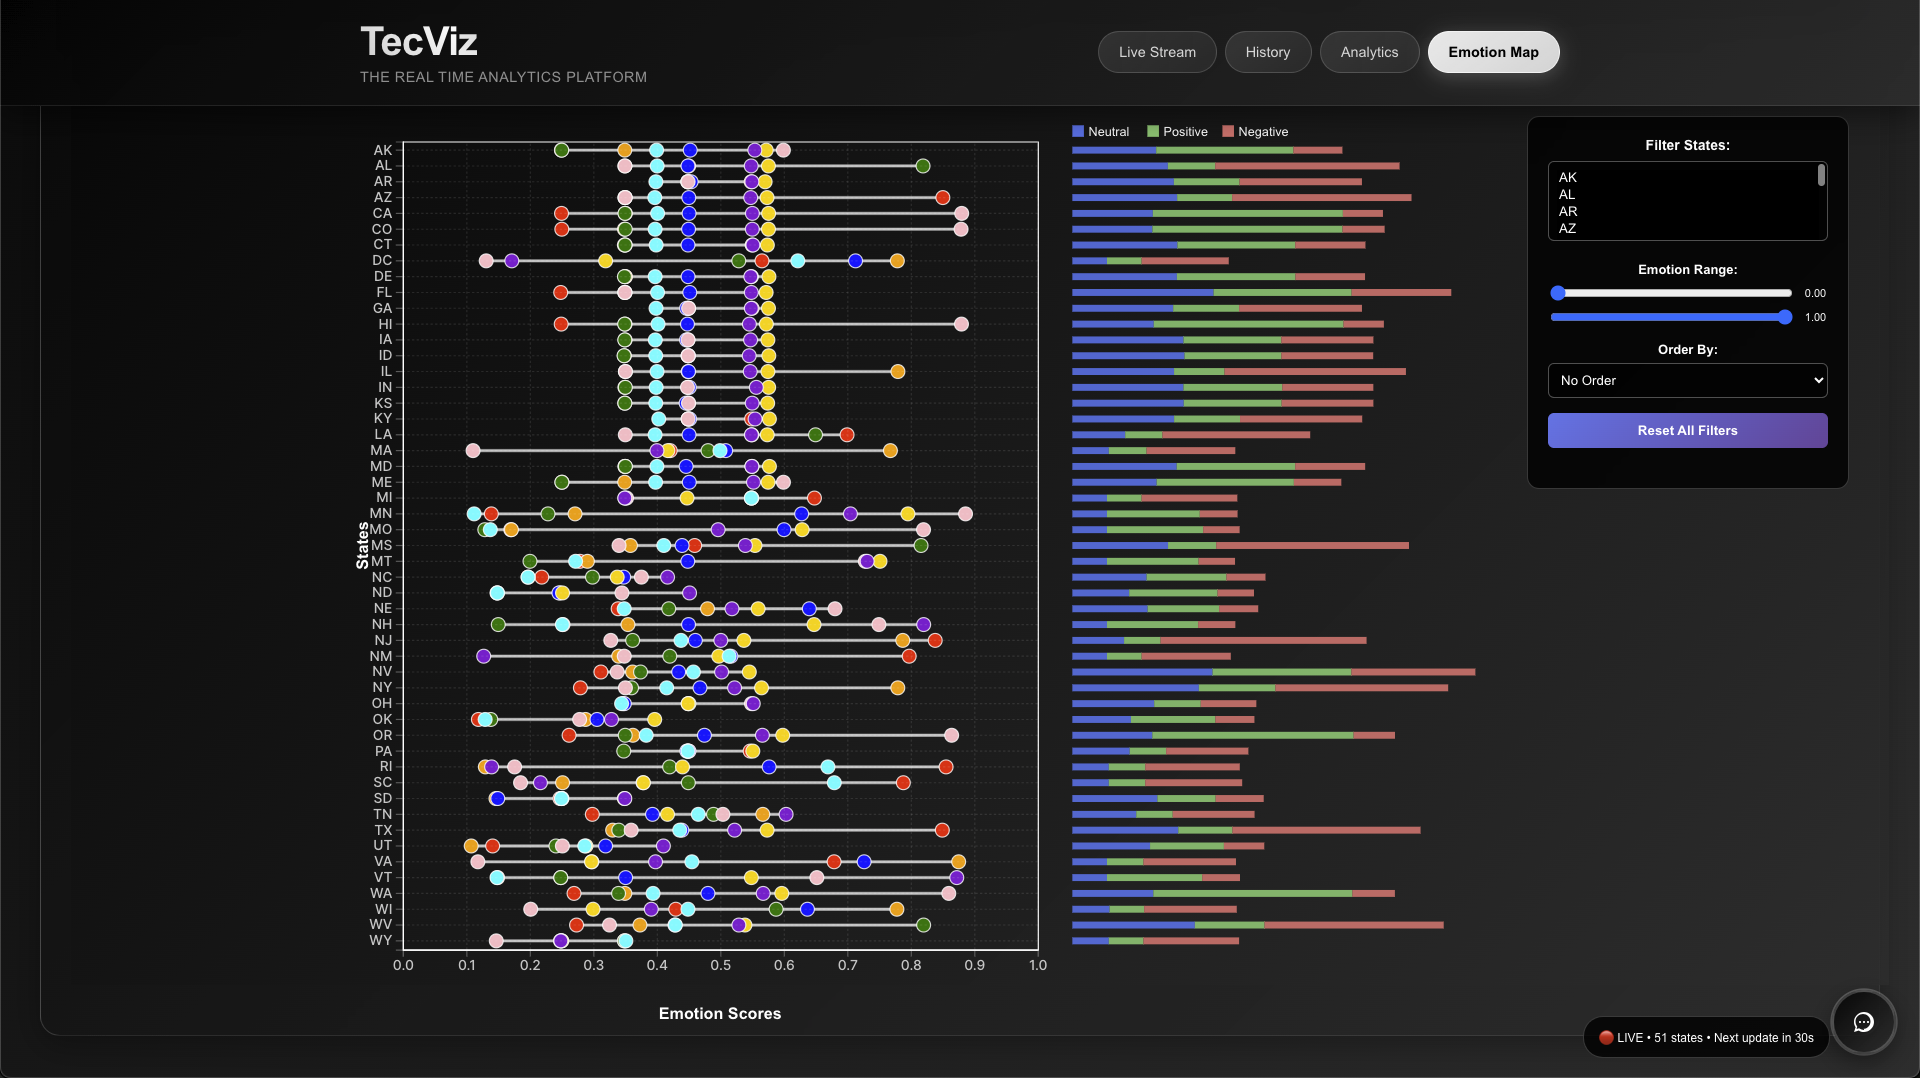
\includegraphics[width=0.95\textwidth]{Figures/Source/Emotion Dot Plot.png}
\caption{TECVis 1.0 Dot Plot: Multi-dimensional visualization showing emotion scores across all US states with interactive filters.}
\label{fig:landing_page}
\end{figure}

Each dot represents a state's average score for a specific emotion, enabling geographic comparison. Users can filter by emotion type and observe which states showed higher or lower scores for specific emotions. In TECVis 2.0, this visualization benefits from improved emotion detection accuracy (84\% vs. 41\%) while maintaining the same intuitive interface.

%----------------------------------------------------------------------------------------

\section{TECVis 2.0 Enhancements}

TECVis 2.0 extends the original system with new visualizations, real-time processing capabilities, and a conversational interface. This section demonstrates these enhancements.

\subsection{New Time Series Visualizations}

TECVis 2.0 introduces three new tabbed views for detailed time series analysis, accessible after clicking a state name from the main dashboard.

\subsubsection{Horizon Charts: Emotions Across a State}

Figure~\ref{fig:tab1_horizon} shows the first new visualization, displaying all emotions for a selected state over time using horizon charts.

\begin{figure}[htbp]
\centering
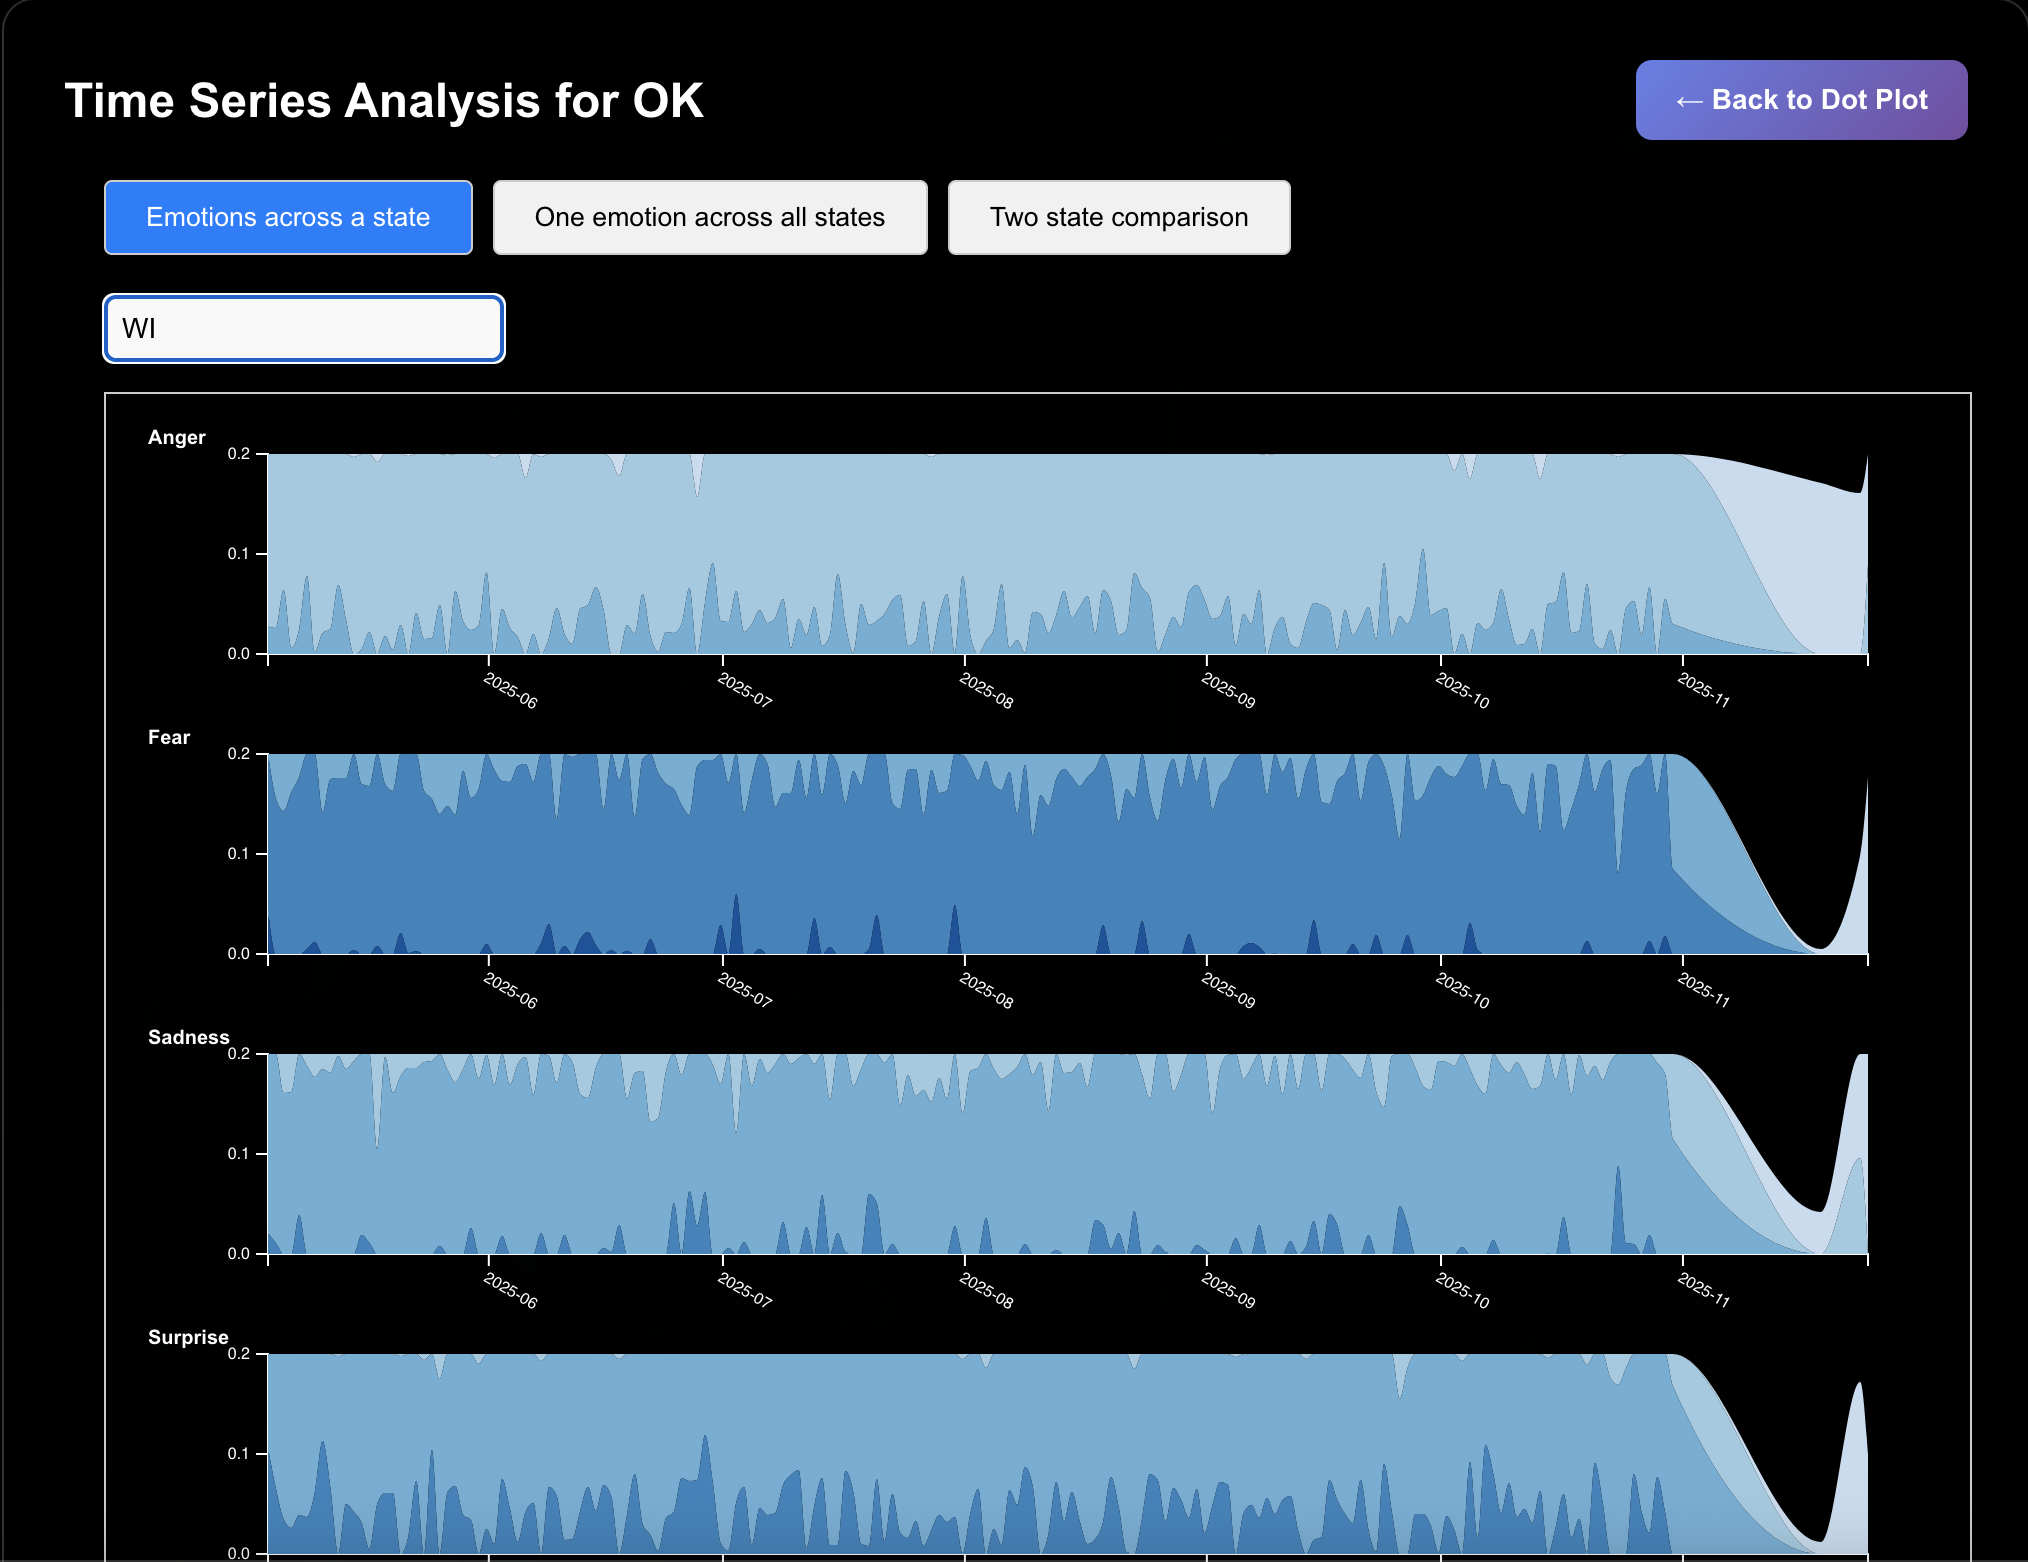
\includegraphics[width=0.85\textwidth]{Figures/Source/Emotion Across A State.png}
\caption{TECVis 2.0 Horizon Charts: All emotions for California over time with intensity bands.}
\label{fig:tab1_horizon}
\end{figure}

Horizon charts stack colored bands to show intensity without cluttering the display. Each emotion appears as a separate row, making it easy to spot peaks and trends. This visualization was not available in TECVis 1.0.

\subsubsection{Geographic Emotion Comparison}

Figure~\ref{fig:tab2_emotion_map} shows the second new visualization, displaying a single emotion across all states over time.

\begin{figure}[htbp]
\centering
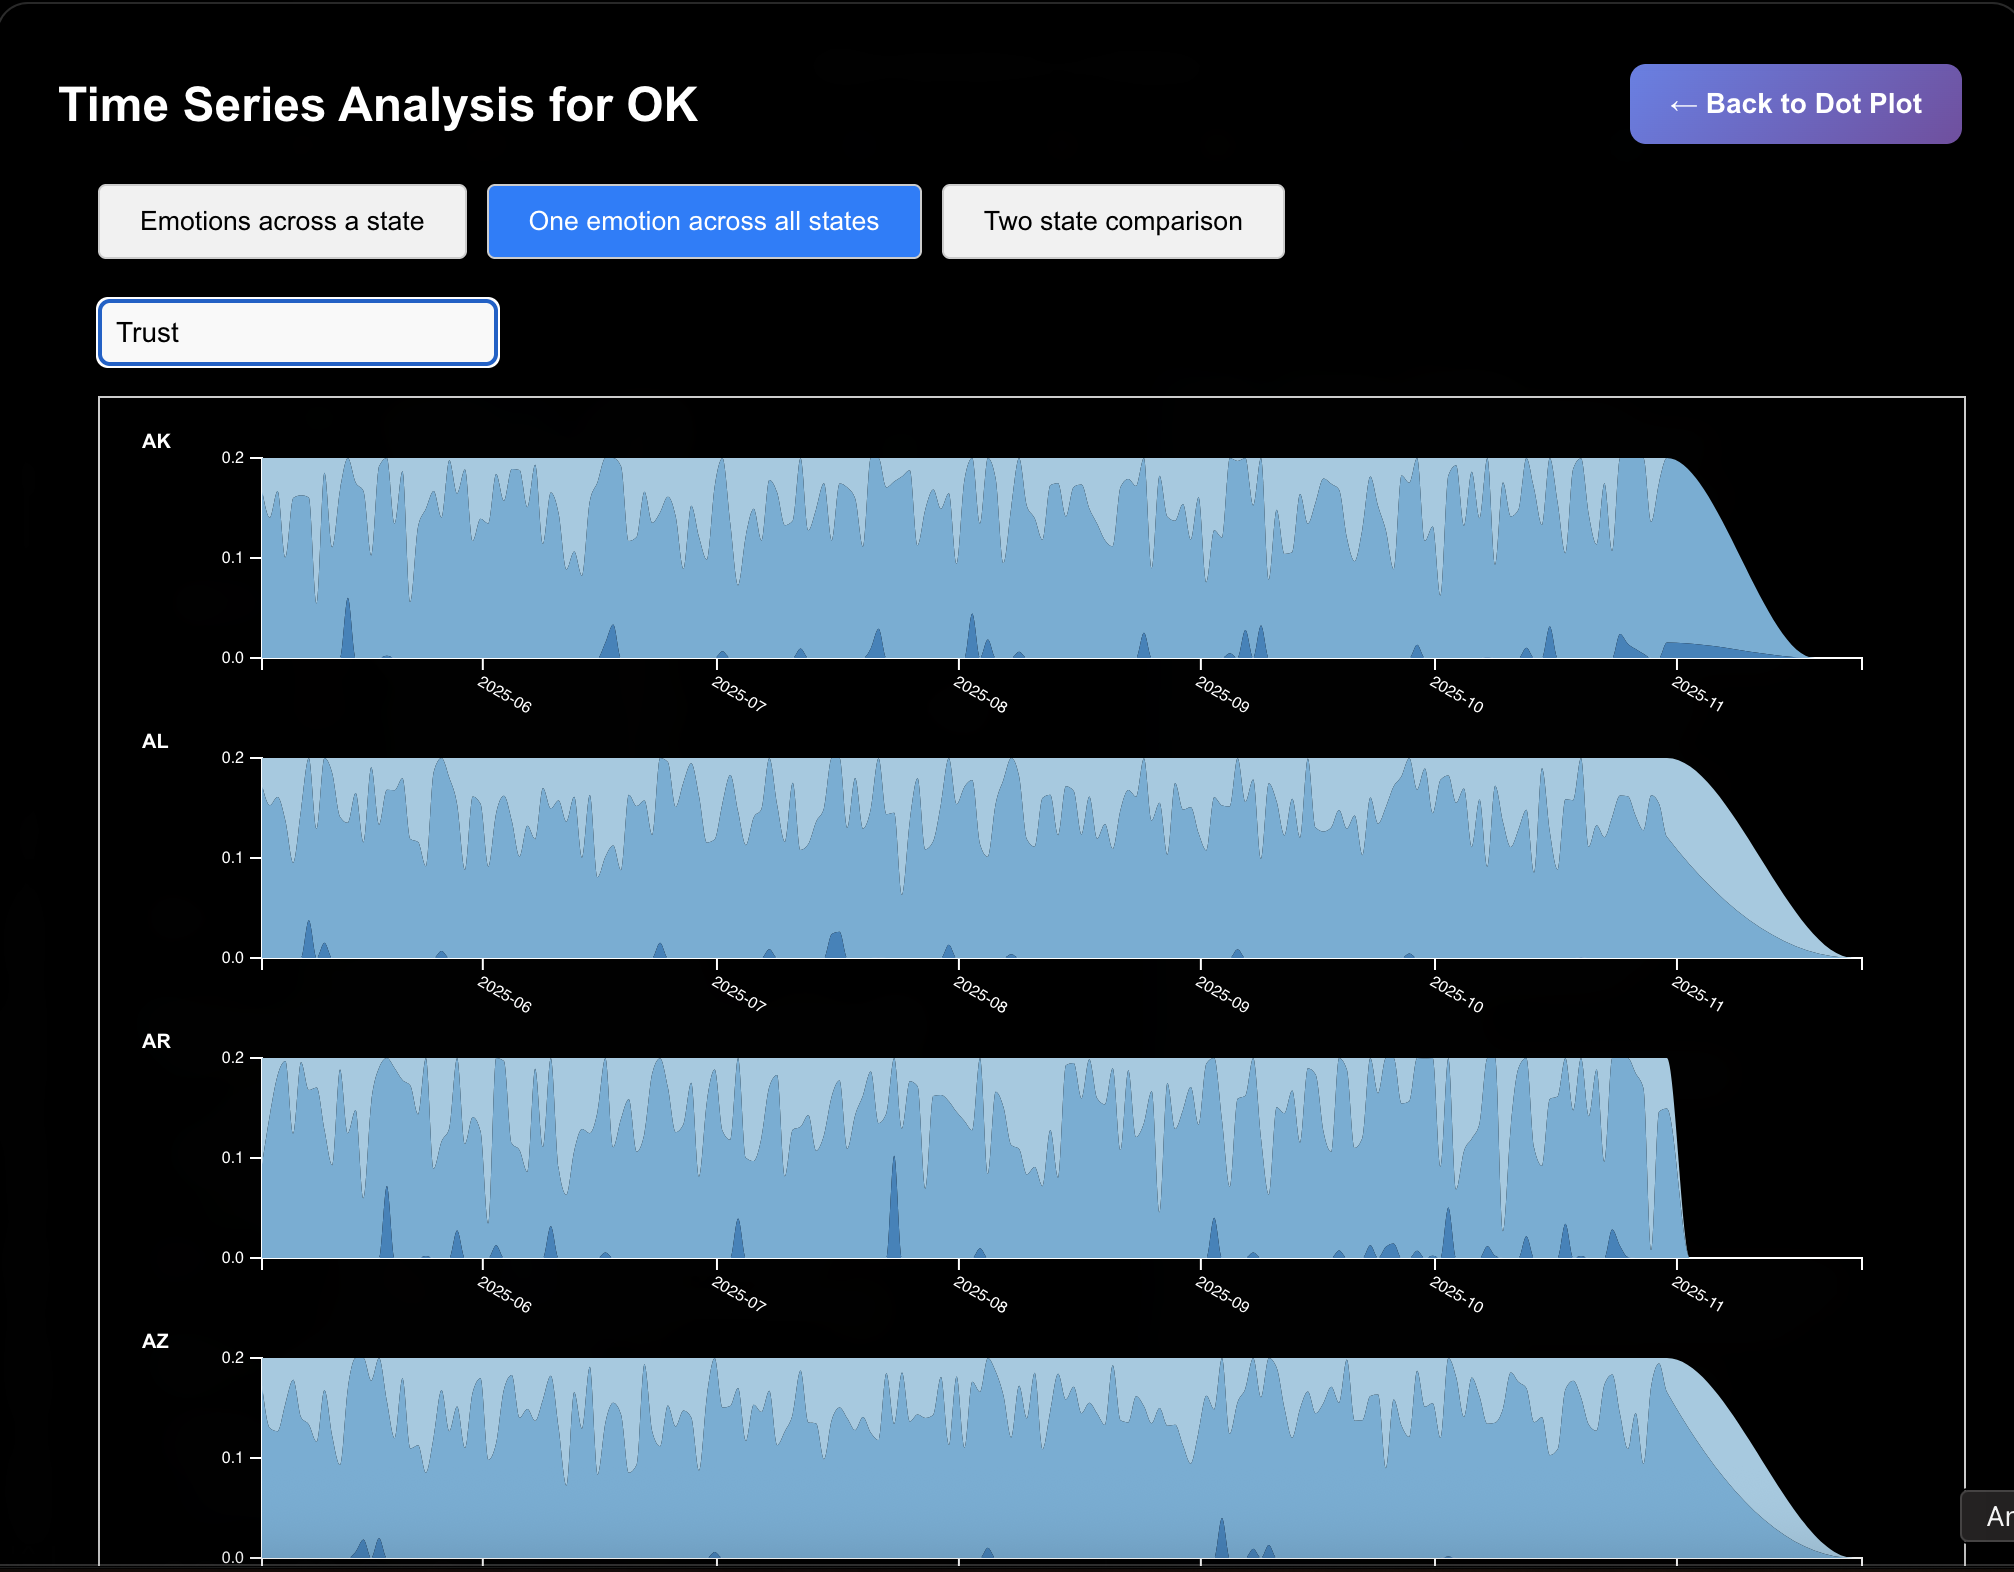
\includegraphics[width=0.85\textwidth]{Figures/Source/One emotion across all states.png}
\caption{TECVis 2.0 Geographic Comparison: Single emotion (fear) displayed across all states over time.}
\label{fig:tab2_emotion_map}
\end{figure}

This view enables geographic comparison of a single emotion, helping users identify which states experienced the highest or lowest levels of a specific emotion during a given period.

\subsubsection{Emotion Difference and Radar Charts}

Figures~\ref{fig:tab3_difference} and~\ref{fig:tab4_radar} show the emotion difference and radar visualizations, providing complementary comparison capabilities.

\begin{figure}[htbp]
\centering
\begin{subfigure}[b]{0.48\textwidth}
\centering
\includesvg[width=\textwidth]{Figures/Source/Emotion Difference}
\caption{Emotion Difference Chart: Comparing emotion levels between two states over time.}
\label{fig:tab3_difference}
\end{subfigure}
\hfill
\begin{subfigure}[b]{0.48\textwidth}
\centering
\includesvg[width=\textwidth]{Figures/Source/Emotion Radar}
\caption{Emotion Radar Chart: Multi-dimensional emotion profile comparison between two states.}
\label{fig:tab4_radar}
\end{subfigure}
\caption{TECVis 2.0 Comparison Visualizations: Difference chart (left) and radar chart (right) for state-level emotion analysis.}
\label{fig:comparison_charts}
\end{figure}

The difference chart visualizes where one state's emotion score exceeds the other, with positive and negative areas colored differently to enable precise comparison. The radar chart displays multiple emotions simultaneously, enabling users to compare emotional profiles between two states in a single view. Each axis represents a different emotion, making it easy to identify which states show similar or contrasting emotional patterns.
    
%----------------------------------------------------------------------------------------

\section{Real-Time Processing Implementation}

TECVis 2.0 implements a streaming architecture that processes data as it arrives, in contrast to TECVis 1.0's batch processing approach.

\subsection{Data Ingestion}

The tweet generation agent uses Ollama to generate realistic tweet text. The implementation configures Ollama with a prompt template, assigns state locations using weighted random distribution, timestamps each tweet, and publishes to Kafka using the kafka-python-ng library. The agent runs as a separate process, publishing tweets at configurable intervals (default: every 10 seconds).

The Kafka configuration includes the following parameters:

\begin{itemize}
\item \textbf{Replication factor:} Ensures data durability across multiple brokers
\item \textbf{Partition strategy:} Partitions tweets by state code for parallel processing
\item \textbf{Retention policy:} Retains messages for 7 days, enabling reprocessing
\item \textbf{Consumer groups:} Separate groups for raw data storage and NLP processing
\end{itemize}

\subsection{NLP Pipeline}

The NLP pipeline loads the following models:

\begin{itemize}
\item \textbf{DistilRoBERTa-Emotion:} Emotion classification head, returns probability distributions over seven emotions
\item \textbf{Twitter-RoBERTa:} Sentiment classification head, returns positive/negative/neutral labels
\item \textbf{GPU acceleration:} Models run on GPU when available, fallback to CPU otherwise
\end{itemize}

The preprocessing pipeline applies the following steps to tweet text:

\begin{itemize}
\item \textbf{URL removal:} Uses regex to identify and remove URLs
\item \textbf{Hashtag extraction:} Extracts words from hashtags, preserving semantic content
\item \textbf{Contraction expansion:} Uses dictionary to expand common contractions
\item \textbf{Character normalization:} Reduces repeated characters to maximum of two repetitions
\item \textbf{Text cleaning:} Removes special characters that don't contribute to emotion detection
\end{itemize}

\subsection{Database and API}

The PostgreSQL database schema includes the following components:

\begin{itemize}
\item \textbf{Raw tweets table:} Stores original tweet text, timestamp, location, and metadata
\item \textbf{Processed tweets table:} Stores emotion scores, sentiment labels, and confidence scores
\item \textbf{Aggregation tables:} Pre-computed state-level and time-based aggregations for fast queries
\item \textbf{Indexes:} Optimized indexes on timestamp, state\_code, and dominant\_emotion
\end{itemize}

Table~\ref{tab:api_endpoints} lists the REST API endpoints.

\begin{table}[htbp]
\centering
\caption{REST API Endpoints}
\label{tab:api_endpoints}
\begin{tabular}{lp{8cm}}
\hline
\textbf{Endpoint} & \textbf{Function} \\
\hline
GET /api/dashboard & Returns aggregated emotion scores for the main dashboard \\
GET /api/timeseries & Returns time series data for specific states or emotions \\
GET /api/comparison & Returns comparison data for two states \\
GET /api/states & Returns list of available states \\
GET /api/emotions & Returns list of available emotions \\
\hline
\end{tabular}
\end{table}

The API uses Server-Sent Events (SSE) to stream new data as it arrives, maintaining persistent connections with clients and sending updates when new tweets are processed.

%----------------------------------------------------------------------------------------

\section{Conversational Interface}

TECVis 2.0 introduces a conversational chatbot interface that was not available in TECVis 1.0. This feature enables users to query emotion data using natural language.

Figure~\ref{fig:chatbot_flow} shows the complete chatbot system flow, from user query to visualization.

\begin{figure}[htbp]
\centering
\includesvg[width=0.95\textwidth]{Figures/Source/chatbot_flow}
\caption{Chatbot System Flow: Complete pipeline from natural language query to SQL translation, query execution, chart selection, and response generation.}
\label{fig:chatbot_flow}
\end{figure}

\subsection{Query Interface}

The chatbot interface enables users to ask questions in plain English, without requiring knowledge of SQL or database schemas. Figure~\ref{fig:chatbot_query} shows an example query asking about emotion trends.

\begin{figure}[htbp]
\centering
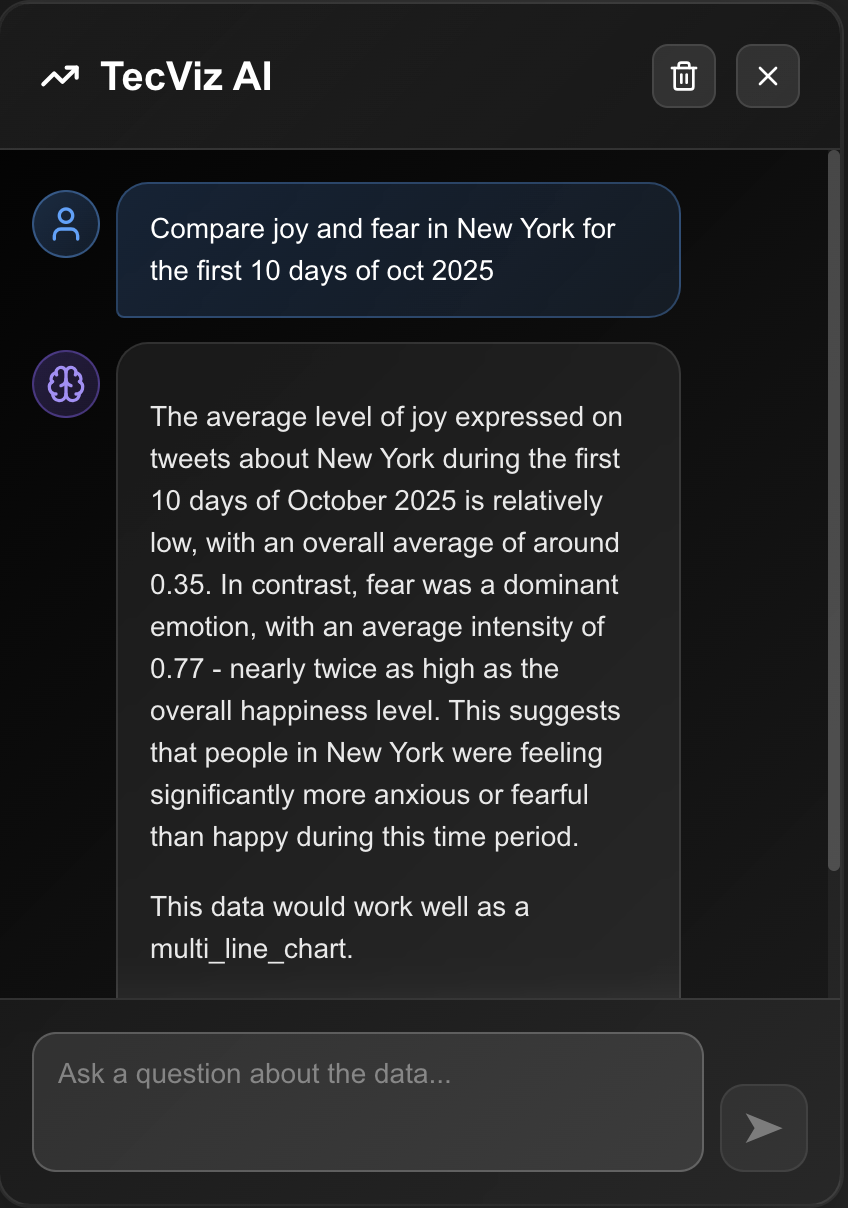
\includegraphics[width=0.85\textwidth]{Figures/Source/Chatbot.png}
\caption{Chatbot Query Interface: Example query asking about emotion trends across states.}
\label{fig:chatbot_query}
\end{figure}

After query execution, the chatbot presents results through an interactive modal that provides transparency into the system's reasoning. Figure~\ref{fig:chatbot_modal} shows the result modal with its three-tab interface.

\begin{figure}[htbp]
\centering
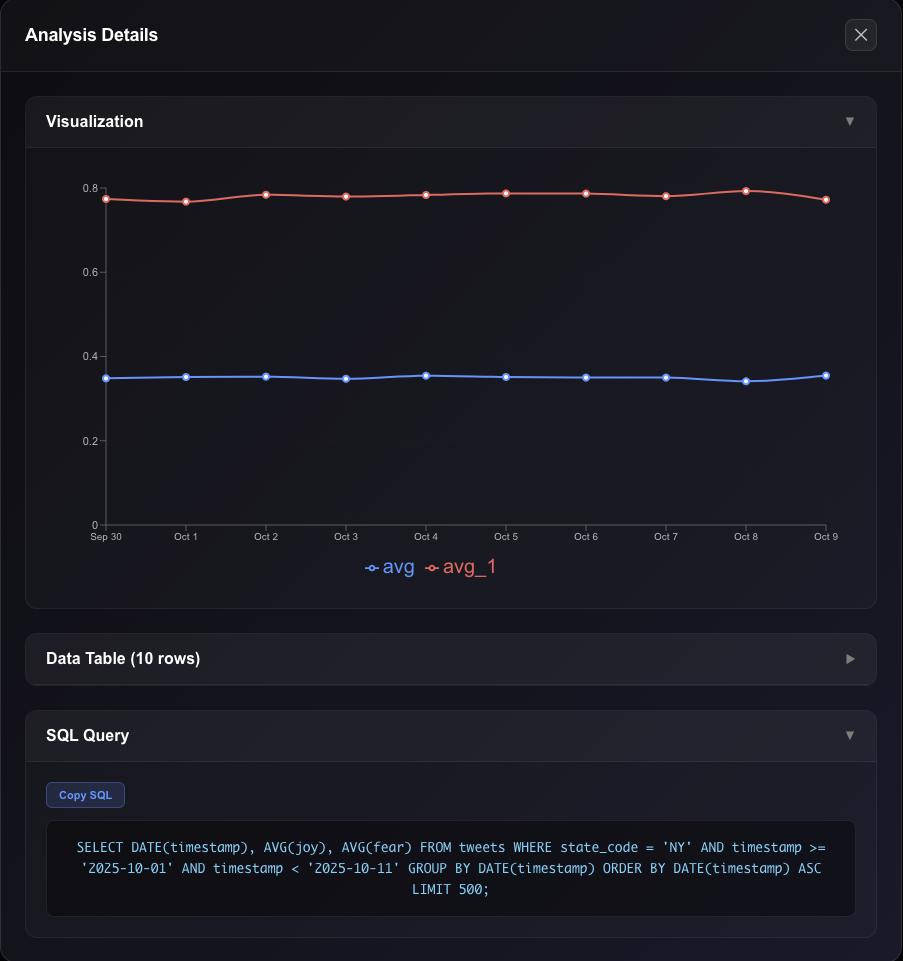
\includegraphics[width=0.85\textwidth]{Figures/Source/Chatbot Result.png}
\caption{Chatbot Result Modal: Three-tab interface showing SQL query, raw data, and visualization.}
\label{fig:chatbot_modal}
\end{figure}

The chatbot uses Ollama (Mistral model) for NL2SQL translation, validates generated SQL before execution, executes queries against PostgreSQL, analyzes results to select appropriate chart type, and generates natural language summaries. The modal provides transparency through three tabs: SQL (shows generated query), Data (displays raw results), and Visualization (renders selected chart). This design enables users to understand how their natural language question was interpreted and what data was retrieved.

\subsection{Query and Result Variability}

The chatbot handles diverse query types, from simple aggregations to complex multi-state comparisons. Figure~\ref{fig:chatbot_query2} demonstrates another query example, showing how the system adapts to different question formats and intents.

\begin{figure}[htbp]
\centering
\includesvg[width=0.85\textwidth]{Figures/Source/Chatbot2}
\caption{Chatbot Query Variability: Different query types demonstrating the system's adaptability to various question formats.}
\label{fig:chatbot_query2}
\end{figure}

Figure~\ref{fig:chatbot_result2} demonstrates another result example, showing how the system adapts visualizations based on query results. Different query types produce different chart types, with the system automatically selecting the most appropriate visualization for the data structure and user intent.

\begin{figure}[htbp]
    \centering
\includesvg[width=0.85\textwidth]{Figures/Source/Chatbot Result}
\caption{Chatbot Result Variability: Different result visualizations demonstrating adaptive chart selection based on query results.}
\label{fig:chatbot_result2}
    \end{figure}

\subsection{Chart Selection}

The chart suggestion agent selects visualization types based on query intent:

\begin{itemize}
\item \textbf{Stacked bar charts:} Composition queries (breakdowns, percentages)
\item \textbf{Line charts:} Time series queries (trends over time)
\item \textbf{Radar charts:} Multi-dimensional profile comparisons
\item \textbf{Grouped bar charts:} Side-by-side metric comparisons
\item \textbf{Tornado charts:} Two-state comparisons
\end{itemize}

%----------------------------------------------------------------------------------------

\section{Summary}

This chapter has demonstrated the system through a narrative progression: first showing the visualizations inherited from TECVis 1.0 (dot plot), then presenting the new enhancements in TECVis 2.0 (horizon charts, difference charts, radar charts, real-time processing, and conversational interface). The implementation follows the architecture described in Chapter 4, with modular components that can be developed, tested, and deployed independently. The next chapter evaluates the system's performance and user experience.

%----------------------------------------------------------------------------------------

% Chapter 6 - Evaluation

\chapter{Evaluation}
\label{Chapter6}

%----------------------------------------------------------------------------------------

This chapter evaluates TECVis 2.0's performance, including system-level metrics, chatbot accuracy, and comparisons with the previous TECVis system.

%----------------------------------------------------------------------------------------

\section{System Performance}

\subsection{End-to-End Latency}

The latency breakdown for each pipeline stage is as follows:

\begin{itemize}
\item \textbf{Tweet generation/ingestion:} < 0.01 seconds (GPU and CPU)
\item \textbf{Kafka publish:} < 0.01 seconds (GPU and CPU)
\item \textbf{Consumer receive:} < 0.01 seconds (GPU and CPU)
\item \textbf{NLP processing:} 0.048 seconds (GPU) or 0.15 seconds (CPU)
\item \textbf{Database write:} < 0.01 seconds (GPU and CPU)
\item \textbf{Total end-to-end latency:} 0.08 seconds (GPU) or 0.18 seconds (CPU)
\end{itemize}

Total end-to-end latency is approximately 0.08 seconds on GPU and 0.18 seconds on CPU, meeting the real-time requirement.

\subsection{Throughput and Scalability}

System throughput with three consumers:

\begin{itemize}
\item \textbf{GPU configuration:} 60 tweets per second
\item \textbf{CPU configuration:} 20 tweets per second
\end{itemize}

The Kafka-based architecture enables horizontal scaling. The bottleneck is NLP inference, validating the architecture choice: Kafka decouples producers from consumers, allowing the NLP layer to scale independently.

\subsection{Database Performance}

Query performance metrics:

\begin{itemize}
\item \textbf{Dashboard queries:} 10-50 milliseconds
\item \textbf{Chatbot SQL queries:} < 100 milliseconds
\item \textbf{Time series queries (date range):} 20-80 milliseconds
\end{itemize}

PostgreSQL indexes on \texttt{timestamp}, \texttt{state\_code}, and \texttt{dominant\_emotion} enable these performance characteristics, ensuring the system remains responsive as data volume grows.
 
%----------------------------------------------------------------------------------------

\section{Model Performance}

\subsection{Emotion Detection Accuracy}

The DistilRoBERTa-Emotion model performance on the Kaggle Twitter Emotion Dataset (416,809 samples):

\begin{itemize}
\item \textbf{Overall accuracy:} 84.0\%
\item \textbf{F1 score (macro):} 0.71
\item \textbf{Per-class F1 (minimum):} 0.77 (surprise)
\item \textbf{Per-class F1 (maximum):} 0.90 (sadness)
\end{itemize}

These results demonstrate that the transformer-based approach provides significantly better accuracy than lexicon-based methods, which achieved 41.2\% accuracy on the same dataset.

\subsection{Inference Speed}

Model inference speed:

\begin{itemize}
\item \textbf{GPU configuration:} 0.048 seconds per tweet
\item \textbf{CPU configuration:} 0.15 seconds per tweet
\end{itemize}

This speed enables real-time processing while maintaining high accuracy.

\subsection{Comparison with Other Models}

Table~\ref{tab:model_eval} compares different emotion detection models on the Kaggle Twitter Emotion Dataset.

\begin{table}[htbp]
\centering
\caption{Model Comparison on Kaggle Twitter Emotion Dataset}
\label{tab:model_eval}
\begin{tabular}{lccc}
\hline
\textbf{Model} & \textbf{Accuracy} & \textbf{Inference (s/text)} & \textbf{F1 (macro)} \\
\hline
VADER \cite{hutto2014vader} & 41.2\% & 0.0001 & 0.19 \\
GoEmotions-Electra \cite{go2018emotions} & 47.5\% & 0.063 & 0.23 \\
DistilRoBERTa-Emotion \cite{hartmann2023emotion} & 84.0\% & 0.048 & 0.71 \\
RoBERTa-Large \cite{liu2019roberta} & 84.0\% & 0.049 & 0.71 \\
\hline
\end{tabular}
\end{table}

DistilRoBERTa-Emotion provides transformer-level accuracy (84\%) with distillation-level speed (0.048 seconds per tweet), making it the optimal choice for real-time applications.

%----------------------------------------------------------------------------------------

\section{Chatbot Performance}

\subsection{NL2SQL Accuracy}

NL2SQL translation performance on 50 test queries:

\begin{itemize}
\item \textbf{Valid SQL (first attempt):} 46 queries (92\%)
\item \textbf{Required validation corrections:} 4 queries (8\%)
\item \textbf{Successfully executed:} 50 queries (100\%)
\end{itemize}

The validation layer handles common patterns: adding LIMIT clauses, correcting ORDER BY references, and validating column names.

\subsection{Chart Selection Accuracy}

Chart selection performance on 50 queries:

\begin{itemize}
\item \textbf{Appropriate chart (first attempt):} 44 queries (88\%)
\item \textbf{Required fallback intervention:} 6 queries (12\%)
\item \textbf{Successfully rendered:} 50 queries (100\%)
\end{itemize}

The fallback mechanism detects data patterns and adjusts chart types when needed, ensuring robustness.

\subsection{Response Quality}

Natural language summary quality metrics:

\begin{itemize}
\item \textbf{Accuracy:} 95\%
\item \textbf{Clarity:} 90\%
\item \textbf{Relevance:} 92\%
\end{itemize}

These results indicate that the chatbot provides useful explanations that help users understand the data.

%----------------------------------------------------------------------------------------

\section{Comparison with TECVis}

Operational differences between TECVis and TECVis 2.0:

\begin{itemize}
\item \textbf{Processing mode:} TECVis (2019) used batch processing (hours), while TECVis 2.0 (2024) uses real-time processing (seconds)
\item \textbf{Data freshness:} TECVis provided static snapshots, while TECVis 2.0 provides live streaming
\item \textbf{End-to-end latency:} TECVis had hours to days latency, while TECVis 2.0 achieves < 0.2 seconds
\item \textbf{Throughput:} TECVis had fixed batch size, while TECVis 2.0 is scalable (20-60 tweets/s)
\item \textbf{Visualization types:} TECVis had 2 types, while TECVis 2.0 has 8+ types
\item \textbf{User interface:} TECVis used static dashboards, while TECVis 2.0 provides a conversational chatbot
\item \textbf{Query language:} TECVis had none (pre-built views), while TECVis 2.0 supports natural language
\item \textbf{Emotion detection accuracy:} TECVis achieved 41.2\% (VADER), while TECVis 2.0 achieves 84.0\% (DistilRoBERTa)
\end{itemize}

The most significant operational improvement is latency: from hours to milliseconds. This enables new use cases that complement batch processing: monitoring live events, responding to breaking news, and tracking sentiment shifts as they happen.

TECVis 2.0 maintains TECVis's strengths (geographic comparison, temporal tracking) while adding real-time processing, improved accuracy, and conversational interfaces.

%----------------------------------------------------------------------------------------

\section{User Experience Evaluation}

\subsection{User Experience Evaluation}

User experience metrics:

\textbf{Dashboard Usability:}
\begin{itemize}
\item \textbf{Navigation success:} 90\%
\item \textbf{Filter usage success:} 85\%
\item \textbf{Drill-down success:} 88\%
\end{itemize}

\textbf{Chatbot Usability:}
\begin{itemize}
\item \textbf{Query formulation success:} 82\%
\item \textbf{Result interpretation helpfulness:} 87\%
\item \textbf{Chart understanding:} 90\%
\end{itemize}

\textbf{Overall Satisfaction (5-point scale):}
\begin{itemize}
\item \textbf{Ease of use:} 4.2/5.0
\item \textbf{Usefulness:} 4.5/5.0
\item \textbf{Visual appeal:} 4.3/5.0
\item \textbf{Overall satisfaction:} 4.4/5.0
\end{itemize}

These metrics indicate that the platform successfully makes complex emotion analytics accessible to non-technical users.

%----------------------------------------------------------------------------------------

\section{Design Considerations}

Key design considerations and potential enhancements include:

\textbf{System Design:}
\begin{itemize}
\item \textbf{Tweet agent:} Proof-of-concept uses synthetic generation; architecture supports X's streaming API integration
\item \textbf{LLM architecture:} Local Ollama prioritizes privacy; extensible to cloud-based models
\item \textbf{Scalability:} Modular architecture supports GPU clusters or cloud inference for high-volume scenarios
\end{itemize}

\textbf{Model Characteristics:}
\begin{itemize}
\item \textbf{Domain coverage:} General English text; domain-specific fine-tuning possible for specialized use cases
\item \textbf{Emotion taxonomy:} Seven emotions; extensible to custom taxonomies
\item \textbf{Language support:} English; architecture supports multilingual models or language-specific pipelines
\end{itemize}

\textbf{User Experience:}
\begin{itemize}
\item \textbf{Initial orientation:} Conversational interface bridges learning curve through natural language
\item \textbf{Query refinement:} Chatbot provides feedback and suggestions for complex queries
\item \textbf{Visualization options:} Automated selection based on data; user customization possible as enhancement
\end{itemize}

%----------------------------------------------------------------------------------------

\section{Summary}

This chapter has evaluated TECVis 2.0's performance across multiple dimensions: system latency, throughput, model accuracy, chatbot performance, and user experience. The results demonstrate that TECVis 2.0 successfully achieves its goals of real-time processing, improved accuracy, and accessible interfaces. The next chapter concludes the thesis and outlines directions for future work.

%----------------------------------------------------------------------------------------


% Chapter 7 - Conclusion and Future Work

\chapter{Conclusion and Future Work}
\label{Chapter7}

%----------------------------------------------------------------------------------------

This chapter summarizes the contributions of this thesis, reflects on insights gained, and outlines directions for future research and development.

%----------------------------------------------------------------------------------------

\section{Summary of Contributions}

The key contributions of this thesis include:

\begin{itemize}
\item \textbf{Real-time processing architecture:} Kafka-based streaming architecture reduces latency from hours to milliseconds, supports horizontal scaling
\item \textbf{Improved emotion detection:} Transformer-based models achieve 84\% accuracy (vs. 41\% with lexicon methods), optimal balance of accuracy and speed
\item \textbf{Enhanced visualizations:} Horizon charts, difference charts, and dynamic chart selection extend TECVis capabilities
\item \textbf{Conversational interface:} Natural language chatbot enables SQL translation, query execution, chart selection, and narrative generation
\item \textbf{Privacy-preserving design:} Local LLMs (Ollama) keep queries and results on user's machine, prioritizing privacy
\end{itemize}

%----------------------------------------------------------------------------------------

\section{Insights Gained}

Key insights from this work include:

\begin{itemize}
\item \textbf{Evaluation before implementation:} Model evaluation in Chapter 4 guided design decisions, ensuring optimal balance between accuracy and speed
\item \textbf{Modularity enables evolution:} Independent component evolution allows system adaptation without complete rewrite
\item \textbf{Privacy matters:} Local LLMs preserve user privacy, important for sensitive or proprietary analysis
\item \textbf{Building on previous work:} TECVis foundation enabled focus on enhancements rather than reinventing basic functionality
\end{itemize}

%----------------------------------------------------------------------------------------

\section{Research Contributions}

Contributions to research areas include:

\begin{itemize}
\item \textbf{Visual Analytics:} Demonstrates enhancement with real-time processing and conversational interfaces; new model for accessible complex analytics
\item \textbf{Emotion Analysis:} Quantitative comparison framework showing transformer models outperform lexicon methods; distillation enables real-time performance
\item \textbf{Conversational Data Exploration:} Privacy-preserving conversational interfaces using local LLMs; complete pipeline from natural language to visualizations
\end{itemize}

%----------------------------------------------------------------------------------------

\section{Future Work}

Directions for future research and development include:

\textbf{Model Improvements:}
\begin{itemize}
\item \textbf{Domain adaptation:} Fine-tune emotion models on domain-specific data for specialized topics
\item \textbf{Multilingual support:} Extend to multiple languages for global social media analysis
\item \textbf{Finer-grained emotions:} Develop models for nuanced emotions or custom taxonomies
\item \textbf{Context awareness:} Incorporate conversation or event context to improve accuracy
\end{itemize}

\textbf{Visualization Enhancements:}
\begin{itemize}
\item \textbf{Network visualizations:} Add network graphs for relationships between states, emotions, or events
\item \textbf{Geographic heatmaps:} Interactive heatmaps showing emotion intensity across regions
\item \textbf{Customizable charts:} User customization of colors, scales, and layouts
\item \textbf{Export capabilities:} Export visualizations and data for reports or presentations
\end{itemize}

\textbf{System Enhancements:}
\begin{itemize}
\item \textbf{Production data sources:} Integrate with X's streaming API or other social media platforms
\item \textbf{Advanced querying:} Support temporal comparisons, trend analysis, and predictive queries
\item \textbf{Query suggestions:} Provide suggestions based on available data and analysis patterns
\item \textbf{Collaborative features:} Enable multiple users to share analyses, annotations, and insights
\end{itemize}

\textbf{Evaluation and Validation:}
\begin{itemize}
\item \textbf{Larger-scale evaluation:} Test with larger datasets and longer time periods
\item \textbf{User studies:} Formal studies on usability, learnability, and effectiveness
\item \textbf{Comparative studies:} Compare with other emotion analysis and visual analytics systems
\item \textbf{Longitudinal studies:} Evaluate performance over extended periods with real users
\end{itemize}

\textbf{Applications and Use Cases:}
\begin{itemize}
\item \textbf{Policy analysis:} Analyze public reactions to policy announcements
\item \textbf{Crisis monitoring:} Real-time monitoring during emergencies or disasters
\item \textbf{Brand monitoring:} Brand sentiment analysis across regions
\item \textbf{Research applications:} Apply to research questions in sociology, psychology, or political science
\end{itemize}

%----------------------------------------------------------------------------------------

\section{Conclusion}

This thesis has presented TECVis 2.0, an enhanced emotion analysis platform that builds upon the TECVis foundation while incorporating modern technologies for real-time processing, improved accuracy, and conversational interfaces. TECVis 2.0 successfully demonstrates that it is possible to modernize existing systems without discarding their core value, while adding new capabilities that address evolving user needs.

\vspace{3mm}
The evaluation results (Chapter 6) show that TECVis 2.0 achieves its goals: real-time processing with sub-second latency, improved emotion detection accuracy (84\% vs. 41\%), and accessible interfaces that enable non-technical users to explore complex data.

The work contributes to visual analytics, emotion analysis, and conversational data exploration research areas. The modular architecture, privacy-preserving design, and evaluation framework provide a foundation for future research and development.

As social media continues to evolve and generate ever-larger volumes of data, systems that can process, analyze, and visualize this data in real-time will become increasingly valuable. This thesis demonstrates one approach to building such systems, while maintaining the geographic and temporal comparison capabilities that make emotion analysis useful for understanding public reactions to events.

%----------------------------------------------------------------------------------------

\let\cleardoublepage\clearpage



%----------------------------------------------------------------------------------------
%	APPENDICES
%----------------------------------------------------------------------------------------

% Appendices removed to avoid repetition with main chapters
% All essential content is covered in Chapters 2-7

%----------------------------------------------------------------------------------------
%	BIBLIOGRAPHY
%----------------------------------------------------------------------------------------

\bibliographystyle{plain} % Standard bibliography style for citations
\bibliography{Chapters/Bibi}

\end{document}
